%\documentclass[ number=5
			   ,series=sidl
			   ,isbn=xxx-x-xxxxxx-xx-x
			   ,url=http://langsci-press.org/catalog/book/17
			   ,output=long   % long|short|inprep              
			   %,blackandwhite
			   %,smallfont
			   ,draftmode   
			  ]{LSP/langsci}                          

\usepackage{LSP/lsp-styles/lsp-gb4e}		% verhindert Komma bei mehrfachen Fußnoten?
                                                      
\usepackage{layout}
\usepackage{lipsum}

%%%% ABOVE FOR LangSciPress %%%%
%%%% ABOVE FOR LangSciPress %%%%
%%%% ABOVE FOR LangSciPress %%%%
\usepackage{libertine}%work-around solution for rendering problematic characters ʦ, ͡  (mostly in \textbf{})

\usepackage{longtable}%Double-lines (\hline\hline) aren’t typeset properly in ‘longtable’-environment across several pages! conflict with other package (maybe xcolor with option ‘tables’?)

\usepackage{multirow}

\usepackage{array} %allows, among other things, centering column content in a table while also specifying width, creates new column style "x" for center-alignment, "y" for right-alignment
\newcolumntype{x}[1]{>{\centering\hspace{0pt}}p{#1}}%
\newcolumntype{y}[1]{>{\raggedleft\hspace{0pt}}p{#1}}%

\usepackage[]{placeins}%using \FloatBarrier command, all floats still floating at that point will be typeset, and cannot cross that boundary. the option here \usepackage[section]{placeins} automatically adds \FloatBarrier to every \section command (only works for \section commands, nothing lower than that!)
%\usepackage{afterpage}%by using the command \afterpage{\clearpage}, all floats will appear, but no new page will be started, thus avoiding bad page breaks around floats

\usepackage{vowel} %for vowel space chart


%%%IS THIS NECESSARY??
%%%%following allows you to refer to footnotes (from http://anthony.liekens.net/index.php/LaTeX/MultipleFootnoteReferences)
%\newcommand{\footnoteremember}[2]{
%  \footnote{#2}
%  \newcounter{#1}
%  \setcounter{#1}{\value{footnote}}
%} \newcommand{\footnoterecall}[1]{
%  \footnotemark[\value{#1}]} 
%%%%previous allows you to refer to footnotes: use \footnoteremember{referenceText} in footnote, then \footnoterecall{referenceText} to refer.

\usepackage{tikz}%
\usetikzlibrary{plothandlers,matrix,decorations.text,shapes.arrows,shadows,chains,positioning,scopes}

\usepackage{synttree} %zeichnet linguistische Bäume
\branchheight{36pt}%sets height between rows in synttree

\usepackage{lscape}%used for landscape pages in index (list of recordings)

\usepackage{polyglossia}
\setmainlanguage{english}


%%%TAKE OUT FOR FINAL VERSION:
%%%TAKE OUT FOR FINAL VERSION:
%%%TAKE OUT FOR FINAL VERSION:

%%%%following readjusts margin text!
%\setlength{\marginparwidth}{20mm}
%\let\oldmarginpar\marginpar
%\renewcommand\marginpar[1]{\-\oldmarginpar[\raggedleft\footnotesize\vspace{-7pt}\color{red}\It{→ #1}]%
%{\raggedright\footnotesize\vspace{-7pt}\color{red}\It{→ #1}}}
%%%%previous readjusts margin text!

%%%The following lines set depth of ToC (LSP default is only 3 levels)!
%%%\renewcommand{\contentsname}{Table of Contents} % überschrift des inhaltsverzeichnisses
%\setcounter{secnumdepth}{5}%sets how deep section/subsection/subsubsections are numbered
%\setcounter{tocdepth}{5}%sets the depth of the ToC %but this doesn't seem to work!!!
%% new commands for LSP book (Grammar of Pite Saami, by J. Wilbur)

\newcommand{\PS}{Pite Saami}
\newcommand{\PSDP}{Pite Saami Documentation Project}
\newcommand{\WLP}{Wordlist Project}

\newcommand{\HANG}{\everypar{\hangindent15pt \hangafter1}}%also useful for table cells
\newcommand{\FB}{\FloatBarrier}%shortcut for this command to print all floats w/o pagebreak

\newcommand{\REF}[1]{(\ref{#1})}%adds parenthesis around the reference number, particularly useful for examples.%\Ref had clash with LSP!
\newcommand{\dline}{\hline\hline}%makes a double line in a table
\newcommand{\superS}[1]{\textsuperscript{#1}}%adds superscript element
\newcommand{\sub}[1]{$_{#1}$}%adds subscript element
\newcommand{\Sc}[1]{\textsc{#1}}%shortcut for small capitals (not to be confused with \sc, which changes the font from that point on)
\newcommand{\It}[1]{\textit{#1}}%shortcut for italics (not to be confused with \it, which changes the font from that point on)
\newcommand{\Bf}[1]{\textbf{#1}}%shortcut for bold (not to be confused with \bf, which changes the font from that point on)
\newcommand{\BfIt}[1]{\textbf{\textit{#1}}}
\newcommand{\BfSc}[1]{\textbf{\textsc{#1}}}
\newcommand{\Tn}[1]{\textnormal{#1}}%shortcut for normal text (undo italics, bolt, etc.)
\newcommand{\MC}{\multicolumn}%shortcut for multicolumn command in tabular environment - only replaces command, not variables!
\newcommand{\MR}{\multirow}%shortcut for multicolumn command in tabular environment - only replaces command, not variables!
\newcommand{\TILDE}{∼}%U+223C %OLD:~}%shortcut for tilde%command ‘\Tilde’ clashes with LSP!%
\newcommand{\BS}{\textbackslash}%backslash
\newcommand{\Red}[1]{{\color{red}{#1}}}%for red text
\newcommand{\Blue}[1]{{\color{blue}{#1}}}%for blue text
\newcommand{\PLUS}{+}%nicer looking plus symbol
\newcommand{\MINUS}{-}%nicer looking plus symbol
%    Was die Pfeile betrifft, kannst Du mal \Rightarrow \mapsto \textrightarrow probieren und dann \mathbf \boldsymbol oder \pbm dazutun.
\newcommand{\ARROW}{\textrightarrow}%→%dieser dicke Pfeil ➜ wird nicht von der LSP-Font unterstützt: %\newcommand{\ARROW}{{\fontspec{DejaVu Sans}➜}}
\newcommand{\DARROW}{\textleftrightarrow}%↔︎%DoubleARROW
\newcommand{\BULLET}{•}%
%%✓ does not exist in the default LSP font!
\newcommand{\CH}{\checkmark}%%\newcommand{\CH}{\fontspec{Arial Unicode MS}✓}%CH as in CHeck
%%following used to separate alternation forms for consonant gradation and umlaut patterns:
\newcommand{\Div}{‑}%↔︎⬌⟷⬄⟺⇔%non-breaking hyphen: ‑  
\newcommand{\QUES}{\textsuperscript{?}}%marks questionable/uncertain forms

\newcommand{\jvh}{\mbox{\It{j}-suffix} vowel harmony}%
%\newcommand{\Ptcl}{\Sc{ptcl} }%just shortcut for glossing ‘particle’
%\newcommand{\ATTR}{{\Sc{attributive}}}%shortcut for ATTRIBUTIVE in small caps
%\newcommand{\PRED}{{\Sc{predicative}}}%shortcut for PREDICATIVE in small caps
%\newcommand{\COMP}{{\Sc{comparative}}}%shortcut for COMPARATIVE in small caps
%\newcommand{\SUPERL}{{\Sc{superlative}}}%shortcut for SUPERLATIVE in small caps
\newcommand{\SG}{{\Sc{singular}}}%shortcut for SINGULAR in small caps
\newcommand{\DU}{{\Sc{dual}}}%shortcut for DUAL in small caps
\newcommand{\PL}{{\Sc{plural}}}%shortcut for PLURAL in small caps
%\newcommand{\NOM}{{\Sc{nominative}}}%shortcut for NOMINATIVE in small caps
%\newcommand{\ACC}{{\Sc{accusative}}}%shortcut for ACCUSATIVE in small caps
%\newcommand{\GEN}{{\Sc{genitive}}}%shortcut for GENITIVE in small caps
%\newcommand{\ILL}{{\Sc{illative}}}%shortcut for ILLATIVE in small caps
%\newcommand{\INESS}{{\Sc{inessive}}}%shortcut for INESSIVE in small caps
\newcommand{\ELAT}{{\Sc{elative}}}%shortcut for ELATIVE in small caps
%\newcommand{\COM}{{\Sc{comitative}}}%shortcut for COMITATIVE in small caps
%\newcommand{\ABESS}{{\Sc{abessive}}}%shortcut for ABESSIVE in small caps
%\newcommand{\ESS}{{\Sc{essive}}}%shortcut for ESSIVE in small caps
%\newcommand{\DIM}{{\Sc{diminutive}}}%shortcut for DIMINUTIVE in small caps
%\newcommand{\ORD}{{\Sc{ordinal}}}%shortcut for ORDINAL in small caps
%\newcommand{\CARD}{{\Sc{cardinal}}}%shortcut for CARDINAL in small caps
%\newcommand{\PROX}{{\Sc{proximal}}}%shortcut for PROXIMAL in small caps
%\newcommand{\DIST}{{\Sc{distal}}}%shortcut for DISTAL in small caps
%\newcommand{\RMT}{{\Sc{remote}}}%shortcut for REMOTE in small caps
%\newcommand{\REFL}{{\Sc{reflexive}}}%shortcut for REFLEXIVE in small caps
%\newcommand{\PRS}{{\Sc{present}}}%shortcut for PRESENT in small caps
%\newcommand{\PST}{{\Sc{past}}}%shortcut for PAST in small caps
%\newcommand{\IMP}{{\Sc{imperative}}}%shortcut for IMPERATIVE in small caps
%\newcommand{\POT}{{\Sc{potential}}}%shortcut for POTENTIAL in small caps
\newcommand{\PROG}{{\Sc{progressive}}}%shortcut for PROGRESSIVE in small caps
\newcommand{\PRF}{{\Sc{perfect}}}%shortcut for PERFECT in small caps
\newcommand{\INF}{{\Sc{infinitive}}}%shortcut for INFINITIVE in small caps
%\newcommand{\NEG}{{\Sc{negative}}}%shortcut for NEGATIVE in small caps
\newcommand{\CONNEG}{{\Sc{connegative}}}%shortcut for CONNEGATIVE in small caps
\newcommand{\ATTRs}{{\Sc{attr}}}%shortcut for ATTR in small caps
\newcommand{\PREDs}{{\Sc{pred}}}%shortcut for PRED in small caps
%\newcommand{\COMPs}{{\Sc{comp}}}%shortcut for COMP in small caps
%\newcommand{\SUPERLs}{{\Sc{superl}}}%shortcut for SUPERL in small caps
\newcommand{\SGs}{{\Sc{sg}}}%shortcut for SG in small caps
\newcommand{\DUs}{{\Sc{du}}}%shortcut for DU in small caps
\newcommand{\PLs}{{\Sc{pl}}}%shortcut for PL in small caps
\newcommand{\NOMs}{{\Sc{nom}}}%shortcut for NOM in small caps
\newcommand{\ACCs}{{\Sc{acc}}}%shortcut for ACC in small caps
\newcommand{\GENs}{{\Sc{gen}}}%shortcut for GEN in small caps
\newcommand{\ILLs}{{\Sc{ill}}}%shortcut for ILL in small caps
\newcommand{\INESSs}{{\Sc{iness}}}%shortcut for INESS in small caps
\newcommand{\ELATs}{{\Sc{elat}}}%shortcut for ELAT in small caps
\newcommand{\COMs}{{\Sc{com}}}%shortcut for COM in small caps
\newcommand{\ABESSs}{{\Sc{abess}}}%shortcut for ABESS in small caps
\newcommand{\ESSs}{{\Sc{ess}}}%shortcut for ESS in small caps
%\newcommand{\DIMs}{{\Sc{dim}}}%shortcut for DIM in small caps
%\newcommand{\ORDs}{{\Sc{ord}}}%shortcut for ORD in small caps
%\newcommand{\CARDs}{{\Sc{card}}}%shortcut for CARD in small caps
\newcommand{\PROXs}{{\Sc{prox}}}%shortcut for PROX in small caps
\newcommand{\DISTs}{{\Sc{dist}}}%shortcut for DIST in small caps
\newcommand{\RMTs}{{\Sc{rmt}}}%shortcut for RMT in small caps
\newcommand{\REFLs}{{\Sc{refl}}}%shortcut for REFL in small caps
\newcommand{\PRSs}{{\Sc{prs}}}%shortcut for PRS in small caps
\newcommand{\PSTs}{{\Sc{pst}}}%shortcut for PST in small caps
\newcommand{\IMPs}{{\Sc{imp}}}%shortcut for IMP in small caps
\newcommand{\POTs}{{\Sc{pot}}}%shortcut for POT in small caps
\newcommand{\PROGs}{{\Sc{prog}}}%shortcut for PROG in small caps
\newcommand{\PRFs}{{\Sc{prf}}}%shortcut for PRF in small caps
\newcommand{\INFs}{{\Sc{inf}}}%shortcut for INF in small caps
\newcommand{\NEGs}{{\Sc{neg}}}%shortcut for NEG in small caps
\newcommand{\CONNEGs}{{\Sc{conneg}}}%shortcut for CONNEG in small caps

\newcommand{\subNP}{{\footnotesize\sub{NP}}}%shortcut for NP (nominal phrase) in subscript
\newcommand{\subVC}{{\footnotesize\sub{VC}}}%shortcut for VC (verb complex) in subscript
\newcommand{\subAP}{{\footnotesize\sub{AP}}}%shortcut for NP (adjectival phrase) in subscript
\newcommand{\subAdvP}{{\footnotesize\sub{AdvP}}}%shortcut for AdvP (adverbial phrase) in subscript
\newcommand{\subPP}{{\footnotesize\sub{PP}}}%shortcut for NP (postpoistional phrase) in subscript

\newcommand{\ipa}[1]{{\fontspec{Linux Libertine}#1}}%specifying font for IPA characters

\newcommand{\SEC}{§}%standardize section symbol and spacing afterwards
%\newcommand{\SEC}{§\,}%

\newcommand{\Nth}{{\footnotesize(\It{n})}}%used in table of numerals in ADJ chapter

%%newcommands for tables in introductionSDL.tex:
\newcommand{\cliticExs}[3]{\Tn{\begin{tabular}{p{28mm} c p{28mm} p{35mm}}\It{#1}&\ARROW &\It{#2} & ‘#3’\\\end{tabular}}}%specifically for the two clitic examples
\newcommand{\Grapheme}[1]{\It{#1}}%formatting for graphemes in orthography tables
%%new command for the section on orthographic examples; syntax: #1=orthography, #2=phonology, #3=gloss
\newcommand{\SpellEx}[3]{\Tn{\begin{tabular}{p{70pt} p{70pt} l}\ipa{/#2/}&\It{#1}& ‘#3’ \\\end{tabular}}}%formatting for orthographic examples (intro-Chapter)


%%new transl tier in gb4e; syntax: #1=free translation (in single quotes), #2=additional comments, z.B. literal meaning:
\newcommand{\Transl}[2]{\trans\Tn{‘#1’ #2}}%new transl tier in gb4e;
\newcommand{\TranslMulti}[2]{\trans\hspace{12pt}\Tn{‘#1’ #2}}%new transl tier in gb4e for a dialog to be included under a single example number


%% used for examples in the Prosody and Segmental phonology chapters:
\newcommand{\PhonGloss}[7]{%PhonGloss = Phonology Gloss;
%pattern: \PhonGloss{label}{phonemic}{phonetic}{orthographic}{gloss}{recording}{utterance}
\ea\label{#1}
\Tn{\begin{tabular}[t]{p{30mm} l}
\ipa{/#2/}	& \It{#4} \\
\ipa{[#3]}	&\HANG ‘#5’\\%no table row can start with square brackets! thus the workaround with \MC
\end{tabular}\hfill\hyperlink{#6}{{\small\textnormal[pit#6#7]}}%\index{Z\Red{rec}!\Red{pit#6}}\index{Z\Red{utt}!\Red{pit#6#7} \Blue{Phon}}
}
\z}
\newcommand{\PhonGlossWL}[6]{%PhonGloss = Phonology Gloss for words from WORDLIST, not from corpus!;
%pattern: \PhonGloss{label}{phonemic}{phonetic}{orthographic}{gloss}{wordListNumber}
\ea\label{#1}
\Tn{\begin{tabular}[t]{p{30mm} l}
\ipa{/#2/}	& \It{#4} \\
\ipa{[#3]}	&\HANG ‘#5’\\%no table row can start with square brackets! thus the workaround with \MC
\end{tabular}\hfill\hyperlink{explExs}{{\small\textnormal[#6]}}%\index{Z\Red{wl}!\Red{#6}\Blue{Phon}}
}
\z}

%%for derivation examples in the derivational morphology chapter!
%syntax: \DerivExam{#1}{#2}{#3}{#4}{#5}{#6}
%#1: base, #2: base-gloss, #3: derived form, #4: derived form gloss, #5: derived form translation, #6: pit-recording, #7: utterance number
\newcommand{\DW}{28mm}%for following three commands, to align arrows throughout
%%%%OLD:
%%%\newcommand{\DerivExam}[7]{\Tn{\begin{tabular}[t]{p{\DW}cl}\It{#1}&\ARROW&\It{#3}\\#2&&#4\\\end{tabular}\hfill\pbox{.3\textwidth}{\hfill‘#5’\\\hbox{}\hfill\hyperlink{pit#6}{{\small\textnormal[pit#6.#7]}}}
%%%%\index{Z\Red{rec}!\Red{pit#6}}\index{Z\Red{utt}!\Red{pit#6.#7}}
%%%}}
%NEW:
\newcommand{\DerivExam}[7]{\Tn{
\begin{tabular}[t]{p{\DW}x{5mm}l}\It{#1}&\ARROW&\It{#3}\\\end{tabular}\hfill‘#5’\\
\hspace{1mm}\begin{tabular}[t]{p{\DW}x{5mm}l}#2&&#4\\\end{tabular}\hfill\hyperlink{pit#6}{{\small\textnormal[pit#6.#7]}}
%\index{Z\Red{rec}!\Red{pit#6}}\index{Z\Red{utt}!\Red{pit#6.#7}}
}}
%%same as above, but supress any reference to a specific utterance
\newcommand{\DerivExamX}[7]{\Tn{
\begin{tabular}[t]{p{\DW}x{5mm}l}\It{#1}&\ARROW&\It{#3}\\\end{tabular}\hfill‘#5’\\
\hspace{1mm}\begin{tabular}[t]{p{\DW}x{5mm}l}#2&&#4\\\end{tabular}\hfill\hyperlink{pit#6}{{\small\textnormal[pit#6]\It{e}}}
%\index{Z\Red{rec}!\Red{pit#6}}\index{Z\Red{utt}!\Red{pit#6.#7}}
}}
\newcommand{\DerivExamWL}[6]{\Tn{
\begin{tabular}[t]{p{\DW}x{5mm}l}\It{#1}&\ARROW&\It{#3}\\\end{tabular}\hfill‘#5’\\
\hspace{1mm}\begin{tabular}[t]{p{\DW}x{5mm}l}#2&&#4\\\end{tabular}\hfill\hyperlink{explExs}{{\small\textnormal[#6]}}
%\index{Z\Red{wl}!\Red{#6}}
}}


%formatting of corpus source information (after \transl in gb4e-environments):
\newcommand{\Corpus}[2]{\hspace*{1pt}\hfill{\small\mbox{\hyperlink{pit#1}{\Tn{[pit#1.#2]}}}}%\index{Z\Red{rec}!\Red{pit#1}}\index{Z\Red{utt}!\Red{pit#1.#2}}
}%
\newcommand{\CorpusE}[2]{\hspace*{1pt}\hfill{\small\mbox{\hyperlink{pit#1}{\Tn{[pit#1.#2]}}\It{e}}}%\index{Z\Red{rec}!\Red{pit#1}}\index{Z\Red{utt}!\Red{pit#1.#2}\Blue{-E}}
}%
%%as above, but necessary for recording names which include an underline because the first variable in \href understands _ but the second variable requires \_
\newcommand{\CorpusLink}[3]{\hspace*{1pt}\hfill{\small\mbox{\hyperlink{pit#1}{\Tn{[pit#2.#3]}}}}%\index{Z\Red{rec}!\Red{pit#2}}\index{Z\Red{utt}!\Red{pit#2.#3}}
}%
%%as above, but for newer recordings which begin with sje20 instead of pit
\newcommand{\CorpusSJE}[2]{\hspace*{1pt}\hfill{\small\mbox{\hyperlink{sje20#1}{\Tn{[sje20#1.#2]}}}}%\index{Z\Red{rec}!\Red{sje20#1}}\index{Z\Red{utt}!\Red{sje20#1.#2}}
}%
\newcommand{\CorpusSJEE}[2]{\hspace*{1pt}\hfill{\small\mbox{\hyperlink{sje20#1}{\Tn{[sje20#1.#2]}}\It{e}}}%\index{Z\Red{rec}!\Red{sje20#1}}\index{Z\Red{utt}!\Red{sje20#1.#2}\Blue{-E}}
}%











%%hyphenation points for line breaks
%%add to TeX file before \begin{document} with:
%%%%hyphenation points for line breaks
%%add to TeX file before \begin{document} with:
%%%%hyphenation points for line breaks
%%add to TeX file before \begin{document} with:
%%\include{hyphenationSDL}
\hyphenation{
ab-es-sive
affri-ca-te
affri-ca-tes
Ahka-javv-re
al-ve-o-lar
com-ple-ments
%check this:
de-cad-es
fri-ca-tive
fri-ca-tives
gemi-nate
gemi-nates
gra-pheme
gra-phemes
ho-mo-pho-nous
ho-mor-ga-nic
mor-pho-syn-tac-tic
or-tho-gra-phic
pho-neme
pho-ne-mes
phra-ses
post-po-si-tion
post-po-si-tion-al
pre-as-pi-ra-te
pre-as-pi-ra-ted
pre-as-pi-ra-tion
seg-ment
un-voiced
wor-king-ver-sion
}
\hyphenation{
ab-es-sive
affri-ca-te
affri-ca-tes
Ahka-javv-re
al-ve-o-lar
com-ple-ments
%check this:
de-cad-es
fri-ca-tive
fri-ca-tives
gemi-nate
gemi-nates
gra-pheme
gra-phemes
ho-mo-pho-nous
ho-mor-ga-nic
mor-pho-syn-tac-tic
or-tho-gra-phic
pho-neme
pho-ne-mes
phra-ses
post-po-si-tion
post-po-si-tion-al
pre-as-pi-ra-te
pre-as-pi-ra-ted
pre-as-pi-ra-tion
seg-ment
un-voiced
wor-king-ver-sion
}
\hyphenation{
ab-es-sive
affri-ca-te
affri-ca-tes
Ahka-javv-re
al-ve-o-lar
com-ple-ments
%check this:
de-cad-es
fri-ca-tive
fri-ca-tives
gemi-nate
gemi-nates
gra-pheme
gra-phemes
ho-mo-pho-nous
ho-mor-ga-nic
mor-pho-syn-tac-tic
or-tho-gra-phic
pho-neme
pho-ne-mes
phra-ses
post-po-si-tion
post-po-si-tion-al
pre-as-pi-ra-te
pre-as-pi-ra-ted
pre-as-pi-ra-tion
seg-ment
un-voiced
wor-king-ver-sion
}\begin{document}\tableofcontents\clearpage

%%%%%%%%%%%%%%%%%%%% ALL THE ABOVE TO BE COMMENTED OUT FOR COMPLETE DOCUMENT! %%%%%%%%%%%


%%%%%%%%%%%%%%%%%%%%%%%%%%%%%% C H A P T E R %%%%%%%%%%%%%%%%%%%%%%%%%%%%%
%%%%%%%%%%%%%%%%%%%%%%%%%%%%%% C H A P T E R %%%%%%%%%%%%%%%%%%%%%%%%%%%%%
\chapter{Prosody}\index{phonology!prosody}\index{phonology!prosodic structure}\label{ProsodicStructure}

\korr{036}This description of the phonology of \PS\ begins with a discussion of prosodic structures before the segmental phonology is described. This choice of ordering is motivated by the important role that prosodic positions play in the distribution of phonemes (in addition to morphophonology). It is useful to first understand the prosodic structure of \PS\ words before looking at their segmental composition here, and later to better understand morphophonology. 

While there are a number of monosyllabic functional words, all \PS\ lexical forms and many functional words are minimally bisyllabic. 
The first two sections (\ref{monosyllabicWords} and \ref{multisyllabicWords}) describe the prosodic structures of these two groups of words.  
Then, utterance-level prosodic phenomena are dealt with in Section \ref{utteranceProsody}.

\section{Monosyllabic word structure}\label{monosyllabicWords}\index{phonology!word structure}
While the majority of \PS\ words are multisyllabic, a small set of functional words are monosyllabic. This set includes, for instance, some interjections, particles, conjunctions and pronouns. These monosyllabic words consist of at least one vowel\footnote{All vowel phonemes except /u͡a/ are attested in monoslyllabic words.} 
and one consonant. This consonant can be in either onset or coda position; it is also possible for both consonant positions to be filled. Consonant clusters are licensed in coda position as well. The possible segmental structure templates for monosyllabic words are listed with examples in Table \vref{monosyllablicTemplates}.\footnote{Here and below, “C” stands for a consonant phoneme and “V” for a vowel phoneme in representations of prosodic template structures.}
\begin{table}\centering
\caption[Segmental templates for monosyllabic words]{Segmental templates for monosyllabic words, including examples}\label{monosyllablicTemplates}
\begin{tabular}{c | c c  l }
			&\MC{2}{c}{\It{examples}}&	\\
\It{template}	& \It{IPA}	& \It{orth}		& \It{gloss} \\\dline
\MR{2}{*}{VC}	&aj		&\It{aj}		& ‘also’ \\
			&ij		&\It{ij}		& ‘isn’t’ (\Sc{neg\BS3sg.prs}) \\\hline
\MR{3}{*}{CV}	&tɛ		&\It{dä}		& ‘then’ \\%\hline
			&lɛ		&\It{lä}		& ‘is’ (be\BS\Sc{3sg.prs})\\%(be\BS{\sc 3sg.prs}) \\
			&jo		&\It{juo}		& ‘already’ \\\hline
\MR{4}{*}{CVC}	&jus		&\It{jus}		& ‘if’ \\
			&taːt		&\It{dát}		& ‘that’ (\Sc{nom.sg}) \\
			&men	&\It{men}		& ‘but’ \\
			&vaɲ		&\It{vanj}		& ‘really’ \\\hline
\MR{2}{*}{CVCC}& kujt	&\It{gujt}		& ‘definitely’ \\
			&mejt	&\It{mejd}		& ‘what’ (\Sc{acc.pl}) \\\hline
\MR{1}{*}{CVCCC}& taːjst	&\It{dájst}		& ‘from these’ (\Sc{dem}-\Sc{prox}-\Sc{elat.pl}) \\\hline
\end{tabular}
\end{table}


\section{Multisyllablic word structure}\label{multisyllabicWords}
All lexical forms and a large number of functional words in \PS\ are minimally bisyllabic. The smallest prosodic segmental structure for multisyllabic words is: \begin{center}VCV\end{center} but larger words are both possible and common, and expand upon this minimal foundation; examples are provided throughout the following discussion. Due to a number of phenomena, it is sensible to posit a phonological domain, which, in following \korr{058}basic principles of phonology \marginpar{get pages?} %(cf. e.g. \citet[280-283]{dixon2010a1})  %citet{GussenJacobs1998}) 
and the prosodic hierarchy %\marginpar{check Pros-Hier for best!}
(cf. e.g. \citet[280-283]{dixon2010a}, \citet{Selkirk1980,Hayes1989,NesporVogel1986}), I will refer to as a \It{foot}. A \PS\ foot is trochaic (counting from left to right) and essentially bisyllabic. Multisyllabic words with an odd number of syllables thus have a final (unstressed) syllable which falls outside of the last foot. 
Whether such a final syllable should belong to the preceding foot or not is a theoretical question which will not be addressed here, but it should be noted that the segments in such syllables are subject to highly restrictive phonotactics compared to the locations within a trochaic foot.\footnote{Cf. Section \ref{Vallophones} on the phonotactics of vowel phonemes.} 
Evidence for the foot as a domain can be found in prosodic \korr{037}(intonation, cf. Section \ref{wordStress}; minimal size restrictions as described here), phonological (segmental restrictions, cf. Chapter \ref{csANDvs}) and morphophonological (stem alternations and vowel harmony, cf. Section \ref{morphophonology}) phenomena. 



\subsection{Word stress}\index{phonology!stress}\label{wordStress}
The initial syllable\footnote{Cf. Section \ref{syllabification} on syllabification.} 
of a \PS\ foot always receives main stress. All other foot-initial syllables receive secondary stress. If a final syllable is odd, it does not receive any stress. As a result, the patterns of stressed and unstressed syllables presented in Figure \vref{trochees} are attested in \PS. 
\begin{figure}
\centering
\begin{tabular}{l}
ˈσσ \\
ˈσσσ \\
ˈσσˌσσ \\
ˈσσˌσσσ \\
ˈσσˌσσˌσσ \\
ˈσσˌσσˌσσσ \\
\end{tabular}
\caption[Trochaic rhythmic patterns in Pite Saami]{Trochaic rhythmic patterns in Pite Saami; here, σ stands for a syllable}\label{trochees}
\end{figure}

\korr{038}Table \vref{syllTempExs} provides some examples for the syllabic structure of words with up to five syllables. 
\begin{table}\centering
\caption{Examples of words with four common syllable structures}\label{syllTempExs}
\begin{tabular}{llll}
\It{pattern}	&\MC{2}{l}{\It{example}}	&\It{gloss}\\\hline
ˈσσ	& /ˈko.le/	&\It{guole}	& fish\BS\Sc{nom.pl}	\\
ˈσσσ	& /ˈbet.na.ka/	&\It{bednaga}	& dog-\Sc{nom.pl}\\
ˈσσˌσσ	& /ˈsaːlp.ma.ˌkirːje/	&\It{sálbmagirrje}	& hymnal\BS\Sc{nom.sg}\\
ˈσσˌσσσ	& /ˈkuh.ka.ˌjol.ki.kijt/	&\It{guhkajuolgigijt}	& long-legger-\Sc{acc.pl} (moose)\\
\hline\end{tabular}
\end{table}
\korr{039}Note that some recent borrowings from Swedish deviate from this structure by having an initial unstressed syllable, as they do in Swedish. For instance, the example in \REF{loanerSylTemp} is from Swedish \It{departement}. 
\PhonGlossWL{loanerSylTemp}{deˈparteˌmɛnːta}{deˈparteˌmɛnːta}{departemännta}{department\BS\Sc{nom.sg}}{3583}

The acoustic correlates for stress \korr{001}seem to be intensity and pitch. 
Note that vowel length does not play a role in stress. Indeed, there are words with a short first vowel and a long second vowel that receive stress on the first syllable, as in the two examples in \REF{have2SGPRSa} and \REF{fishDIM1}.
\PhonGloss{have2SGPRSa}{ˈanaː}{ˈanaː}{aná}{have\BS\Sc{2sg.prs}}{101208}{.246}
\PhonGloss{fishDIM1}{ˈkolaː-ʧ}{ˈku͡ɔlaːʧ}{guolátj}{fish-\Sc{dim}}{110413a}{.067}
However, more detailed analyses is required to fully describe the acous\-tic\--pho\-ne\-tic behavior of word-level stress\korr{039}, including the difference between primary and secondary stress. 


\subsection{Relevant prosodic domains}\label{prosodicDomains}
Due to systematic restrictions on the distribution of a number of segments and consonant clusters as well as to the prosodic domains of morphophonological processes, it is useful to name and describe various prosodic positions for multisyllabic words. The domains themselves are described below, while the relevant phonological restrictions and morphophonological processes are described in the pertinent sections on consonant phonemes (Section \ref{consonants}), vowel phonemes (Section \ref{vowels}) and morphophonology (Section \ref{morphophonology}). Only a very limited number of recent loan words do not adhere to this structure. 
The illustration in Figure \vref{prosodicDomainFigure} shows these prosodic positions, and they are described further below. In the illustration, only segments represented by bold capital letters are obligatory.
%%%new commands for the following figure only:
\newcommand{\Cyes}{{\fontspec{Arial}\Bf{C}}}
\newcommand{\Cno}{{\fontspec{Arial}c}}
\newcommand{\Vyes}{{\fontspec{Arial}\Bf{V}}}
\newcommand{\Vno}{{\fontspec{Arial}v}}
\begin{figure}\centering
\tikzset{terminal/.style={rectangle,minimum size=10mm,rounded corners=1mm,thick,draw=red!50!black!80,top color=white,bottom color=red!40!black!20}}
\tikzset{terminalBIG/.style={rectangle,minimum size=20mm,rounded corners=1mm,thick,draw=red!50!black!80,top color=white,bottom color=red!70!black!20}}
\tikzset{terminalLONG/.style={rectangle,minimum width=55mm,rounded corners=3pt,thick,left color=white,right color=white,middle color=red!50!black!50}}
%\newcommand{\Slant}{anchor=east,xshift=3mm,yshift=4mm}
\begin{tikzpicture}[node distance=1mm]
%boxed in Cs and Vs:
\node (initium1) [terminal] {\Cno\Cno\Cno};\node (Vcenter1) [terminal,right=of initium1] {\Vyes};\node (Ccenter1) [terminal,right=of Vcenter1] {\Cno\Cno\Cyes};\node (latus1) [terminal,right=of Ccenter1] {\Vyes};\node (Cmargin1) [terminal,right=of latus1] {\Cno\Cno\Cno};\node (Vmargin1) [terminal,right=of Cmargin1] {\Vno};\node (finis1) [terminal,right=of Vmargin1] {\Cno\Cno\Cno}; %break between levels
%labels:
\node (initium2) [rotate=65,below=of initium1,anchor=north east,xshift=1mm,yshift=3mm] {foot onset};\node (Vcenter2) [rotate=65,below=of Vcenter1,anchor=north east,xshift=1mm,yshift=3mm] {V1};\node (Ccenter2) [rotate=65,below=of Ccenter1,anchor=north east,xshift=1mm,yshift=3mm] {consonant center};\node (latus2) [rotate=65,below=of latus1,anchor=north east,xshift=1mm,yshift=3mm] {V2};\node (Cmargin2) [rotate=65,below=of Cmargin1,anchor=north east,xshift=1mm,yshift=3mm] {C2};\node (Vmargin2) [rotate=65,below=of Vmargin1,anchor=north east,xshift=1mm,yshift=3mm] {V3};\node (finis2) [rotate=65,below=of finis1,anchor=north east,xshift=1mm,yshift=3mm] {C3};%\node (Ccenter1) [terminalBIG,right=of Vcenter1,xshift=-5mm] {\Huge CCC};
%footification:
\node (foot) [terminalLONG,above=of Ccenter1,anchor=south,xshift=0mm,yshift=0mm] {foot};
\end{tikzpicture}
\caption[Illustration of prosodic domains for segments and the foot]{Illustration of prosodic domains for segments and the foot; segments represented by \Cyes\ and \Vyes\ are obligatory, while \Cno\ and \Vno\ are not.}\label{prosodicDomainFigure}% (based on \cite{Sammallahti1998}:39); this illustration does not reflect any quantity distinctions for these slots.}
\end{figure}

\korr{061}Note that Figure \vref{domainExamples} provides examples of how a word’s segments fill these positions; it may be useful to refer to this to better understand these prosodic domains. 


\subsubsection{Foot}\label{foot}\index{prosodic positions!foot}
A \Bf{foot} in \PS\ is a prosodic unit consisting of a stressed syllable and the following unstressed syllable, and is thus trochaic. Every multi-syllabic \PS\ word consists of at least one foot. 

\subsubsection{Foot onset}\label{footOnset}\index{prosodic positions!onset}
\Bf{Foot onset} position is the first consonant or consonant cluster of a foot. It is not obligatorily filled. 
In Saamic linguistics, this has typically been referred to as the ‘initium’ \korr{059}\citep[cf.][p?p]{Sammallahti1998}.

\subsubsection{V1}\label{v1}\index{prosodic positions!V1}
\Bf{V1} is the first vowel of a foot, and is the peak of the stress-carrying syllable for the foot. It can be long or short, and can be a monophthong or a diphthong. The vowel in the final V1 position\footnote{Only words of four or more syllables can have more than one V1 position.}
 of a word is the location for umlaut and ablaut/\It{j}-harmony (cf. Sections \ref{umlaut} and \ref{VH}). 
In Saamic linguistics, this has been referred to as the ‘vowel center’ \citep[cf.][p?p]{Sammallahti1998}.

\subsubsection{The consonant center}\label{CCent}\is{consonant center}
The \Bf{consonant center} is the consonant or consonants that follow V1 (the initial vowel) and precede V2 (the second vowel), and essentially form the core 
of a foot. Every foot has a consonant center. The final consonant segment of the consonant center is the onset of the second syllable due to syllabification (cf. Section \ref{syllabification}). The final consonant center of a word is the location for consonant gradation. The term ‘consonant center’ is commonly used in Saami linguistics \citep[cf.][p?p]{Sammallahti1998}. 

\subsubsection{V2}\label{v2}\index{prosodic positions!V2}
\Bf{V2} is the second vowel of a foot. It never carries stress. Every foot has a vowel in this position. With the exception of the diphthong phoneme /u͡a/, all vowel phonemes are licensed here. 
In Saamic linguistics, this has been referred to as the ‘latus’ \citep[cf.][p?p]{Sammallahti1998}.

\subsubsection{C2}\label{CMarg}\index{prosodic positions!C2}
\Bf{C2} is the consonant or consonants following V2. It is not obligatorily filled. If it is followed by a V3, then its final segment is resyllabified as the onset of the following syllable. 
In Saamic linguistics, this has also been referred to as the ‘consonant margin’ \citep[cf.][p?p]{Sammallahti1998}.

\subsubsection{V3}\label{v3}\index{prosodic positions!V3}
\Bf{V3} is the unstressed vowel of any syllable following the final foot of a multisyllabic word form, and is thus the last syllable nucleus of a word (when present). Only a limited set of vowel phonemes can occur in this position. If the V3 position is filled, then there is always a consonant margin as well.  
In Saamic linguistics, this has been referred to as the ‘vowel margin’ \citep[cf.][p?p]{Sammallahti1998}.

\subsubsection{C3}\label{c3}\index{prosodic positions!C3}
\Bf{C3} is a consonant or one of a limited set of consonant clusters (cf. Section \ref{CCsWordfinal}) following V3 of a multisyllabic word, and is thus always word-final (when present). It is not obligatorily filled. If the C3 position is filled, then there is always a vowel in V3 and a consonant margin as well. 
In Saamic linguistics, this has been referred to as the \korr{018}‘finis’ \korr{060}\citep[cf.][p?p]{Sammallahti1998}.


\subsubsection{Discussion and examples}\label{exampleFootedness}
Table \vref{domainExamples} provides several examples for \PS\ multisyllablic words and how their segments fill the prosodic domains described above. Note that there are always segments in V1, the consonant center and V2, forming a sort of ‘minimal core.’
\begin{table}\centering
\caption{Examples showing how the segments of \PS\ words fill prosodic domains}\label{domainExamples}
\begin{tabular}{| c || c |c c c| c c c || c |}\hline
		&\MC{7}{c||}{\It{prosodic domains}}							&\\\cline{3-5}
		&\It{foot}	&\MC{3}{c|}{\It{minimal core}}&			&	&	&\\
\It{IPA}	&\It{onset}&\It{V1}&\It{C-center}&\It{V2}&\It{C2} &\It{V3}&\It{C3}&\It{gloss} \\\dline
ane		& 		&a	& n		& e	&		&		&	& have\BS\sc{sg.imp}\\
%eno		& 		&e	& n		& o	&		&		&	& river\BS\sc{nom.pl}\\
pena		&p 		&e	& n		& a	&		&		&	& dog\BS\sc{nom.sg}\\
atne-t	& 		&a	& tn		& e	&t		&		&	& have-\sc{inf}\\
kolːe		&k 		&o	& lː		& e	&		&		&	& fish\BS\sc{nom.sg}\\
kolːaː-j	&k 		&o	& lː		& aː	&j		&		&	& fish-\sc{ill.sg}\\
vaːjpmo	&v		&aː	& jpm	& o	&		&		&	& heart\BS\sc{nom.sg}\\
lu͡akːta-j	&l		&u͡a	& kːt		& a	& j		&		&	& bay-\sc{ill.sg}\\
ʃɲerːa	&ʃɲ		&e	& rː		&a	&		&		&	& rat\BS\sc{nom.sg}\\
uvːata	&		&u	& vː		&a	&t		&a		&	& kiss\BS\sc{2sg.prs}\\
puʰʦu-jta	&p		&u	& ʰʦ		&u	&jt		&a		&	& reindeer-\sc{ill.pl}\\
saːkasta-v	&s 		&aː	& k		& a	&st		&a		&v	& say-\sc{1sg.prs}\\
petnaki-st	&p 		&e	& tn		& a	&k		&i		&st	& dog-\sc{elat.sg}\\
\hline
\end{tabular}
\end{table}
Only the final foot of a word can be followed by a single, odd syllable with V3 and potentially C3 segments. 

Similarly, only the final foot of a word is subject to morphophonological phenomena (cf. Section \ref{morphophonology}). For instance, \It{sálbmagirjje} ‘book of psalms, hymnal’ is a compound consisting of \It{sálbma} ‘psalm’ and \It{girjje} ‘book’. It consists of two feet: \It{sálbma-} and \It{-girjje}. It is not possible to add another syllable (e.g. via suffixation) between these two feet because they belong to the same compound noun. Furthermore, the inflected form for \Sc{acc.sg} is \It{sálbmagirjev}, in which consonant gradation (weakening of /jj/ to /j/) is only triggered in the second foot, even though the first foot undergoes gradation (weakening of the cluster /lpm/ to /lm/) in non-compound environments, cf. \It{sálmav} ‘psalm-\Sc{acc.sg}’. This is illustrated by the word forms in Table \vref{hymnalExample}.
\begin{table}\centering
\caption{Examples showing how the scope of consonant gradation is limited to the final foot of a word}\label{hymnalExample}
\begin{tabular}{|l|l|l|}\hline
\Sc{nom.sg}	&\Sc{acc.sg}		&\It{gloss}	\\\dline
 sálbma		& sálmav		& ‘psalm’	\\\hline
 girrje		& girjev		& ‘book’	\\\hline
 sálbmagirrje	& sálbmagirjev	& ‘hymnal’	\\
			& *sálmagirjev	&		\\\hline
\end{tabular}
\end{table}


\subsection{Syllabification}\label{syllabification}\index{syllabification}
The distribution of vowel phonemes between consonant phoneme slots patterns clearly, particularly with respect to intonation and the distribution of vowel phonemes. 
This, along with the sonority sequencing principle \korr{062}\citep[cf. e.g.][]{Selkirk1984}, indicates that vowels are the nuclei of \PS\ syllables.  
However, the location of syllable boundaries is not as easy to determine; in fact, syllable boundaries are not highly relevant in \PS\ prosody. 

Because the consonant center has by far the widest variety of consonants and consonant combinations of any of the consonant positions, it is best to consider this position first. 
However, although the consonant center spans the preceding and following syllabic nuclei, there is no solid phonotactic or phonological evidence for where the syllable boundary is located inside the consonant center. 
The possible syllabification patterns for the consonant center are listed in Table \vref{syllabificationPatternsInCCent}. 
\newcommand{\HSP}{\hspace*{6pt}}%new command to coordinate spacing in following table only
\begin{table}\centering
\caption{Logically possible syllabification patterns for the consonant center}\label{syllabificationPatternsInCCent}
\begin{tabular}{|c c|}\hline%\centering
\It{C-center segment count}	&\It{possible patterns} \\\hline
one C	& V.CV \HSP VC.V \\%\hline
two Cs	& V.CCV \HSP VC.CV \HSP VCC.V \\
three Cs	& V.CCCV \HSP VC.CCV \HSP VCC.CV \HSP VCCC.V \\\hline
\end{tabular}
\end{table}

Maximizing onsets, the patterns V.CCCV, VC.CCV and V.CCV would create highly unusual onsets (such as /vkŋ/, /pm/ or /vɲ/) unattested in any other onset positions. 
Similarly, trying to maximize codas, the patterns VCCC.V and VCC.V would also result in highly unusual codas (such as /vkŋ/ or /vɲ/) unattested in any other coda positions. 
While the pattern VCC.CV would also create some otherwise unattested codas (such as /vt/ or /rk/), these are phonologically similar to attested word-final codas such as /st/ or /jk/ (also fricative\PLUS plosive and oral-sonorant\PLUS plosive, respectively). 
The patterns VC.CV, V.CV and VC.V result in onsets and codas which are not unusual. However, keeping in mind the far greater diversity of single consonant phonemes licensed in word-initial onset position compared to word-final coda position, syllabification favoring singleton onset consonants results in onsets and codas which most resemble word-initial onsets and word-final codas. Note that even then, onsets and codas in positions other than the consonant center form subsets of the possibilities in consonant center position (with the exception of a few non-native word-onset clusters). It is therefore most plausible that syllables are assigned a single consonant segment as an onset in syllabification. The examples in \REF{have2SGPRSb} through \REF{laughINF}\footnote{Cf. Section \ref{examplesExample} for an explanation of the sources in the examples in the current chapter.} 
show some results of this syllabification for a variety of consonant constellations in the consonant center.
\PhonGlossWL{have2SGPRSb}	{anaː}	{a.naː}		{aná}	{have\BS\Sc{2sg.prs}}	{6278}
\PhonGlossWL{haveINF}		{atne-t}	{at̚.net}		{adnet}	{have-\Sc{inf}}	{0006}
\PhonGloss{bayNOMPL}		{lokta}	{lʊ͡okʰ.ta}		{luokta}	{bay\BS\Sc{nom.pl}}	{080702b}{.54m38s}
%\PhonGlossLongSource{bayNOMPL}		{lokta}	{lʊ͡okʰ.ta}		{luokta}	{bay\BS\Sc{nom.pl}}	{080702b}{.54m38s}
\PhonGlossWL{boxDIM}			{kisto-ʧ}	{kis.toʧ}		{gistotj}	{box-\Sc{dim}}		{6048}
%\PhonGloss{spoonNOMPL}	{piste}	{pis.te}		{biste}	{spoon\BS\Sc{nom.pl}}		{-}
\PhonGlossWL{work1SGPRS}	{parka-v}	{par.kaʋ}		{bargav}	{work-\Sc{1sg.prs}}	{6241}
\PhonGloss{laughINF}		{ʧaːjpma-t}{ʧaːjp̚.matʰ}	{tjájbmat}	{laugh-\Sc{inf}}		{100323a}{.001}

This syllabification preference for a single onset segment can be applied to syllable boundaries outside of the consonant center, as shown in \REF{speakINFa} and \REF{happinessCOMSG}. 
\PhonGlossWL{speakINFa}		{saːkasti-t}	{saː.kas.titʰ}	{ságastit}	{speak-\Sc{inf}}			{1480}
\PhonGlossWL{happinessCOMSG}{ɛvu-jna}	{ɛ.vuj.na}		{ävujna}	{happiness-\Sc{com.sg}}	{4372}

\korr{002}When the consonant center consists of a geminate phoneme (cf. Section \ref{geminateCs}), there is no phonological test which indicates where the syllable boundary is located; 
indeed, this syllable boundary is likely not relevant in \PS\ phonology. With this in mind, a symbolic syllable boundary is postulated somewhere within a phonological geminate; this divides the geminate symbolically into two component parts and results in syllables conforming to a syllable template with a singleton in the onset. In the examples in \REF{whileNOMSG} through \REF{fatherNOMSGa}, this symbolic boundary is placed in the middle of the geminate.
\PhonGlossWL{whileNOMSG}	{pɔtːɔ}	{pɔt̚.tɔ}		{båddå}	{while\BS\Sc{nom.sg}}		{0231}
\PhonGlossWL{nameNOMSG}	{namːa}	{nam.ma}		{namma}	{name\BS\Sc{nom.sg}}		{3433}
\PhonGloss{milkingbowlNOMSG}	{naːʰpːe}	{naːhp̚.pe}	{náhppe}	{milking\_cup\BS\Sc{nom.sg}}	{080621}{.54m38s}
\PhonGlossWL{fatherNOMSGa}		{a:ʰʧːe}	{a:ht̚.ʧe}	{áhttje}	{father\BS\Sc{nom.sg}}{0016}

If a geminate precedes another consonant segment in the consonant cluster, the syllabification border is after the geminate, as in \REF{spoonNOMSG}:
\PhonGlossWL{spoonNOMSG}	{pisːte}	{pisː.te}		{bisste}	{spoon\BS\Sc{nom.sg}}		{0190}

\korr{003}When the final consonant in the consonant center is preaspirated, there is again no test for the location of a syllable boundary, as with geminates. With this in mind, a symbolic boundary is posited between the realization of preaspiration (cf. Section \ref{preaspiration}) and the rest of the preaspirated segment, which results in syllables conforming to a syllable template with a simpleton in the onset. The examples in \REF{houseNOMSGa} and \REF{endNOMSG} show a preaspirated plosive and affricate, respectively, with a syllable boundary indicated between the glottal fricative (preaspiration) and the stop or affricate component.
\PhonGlossWL{houseNOMSGa}	{tɔʰpe}	{tɔh.pe}		{dåhpe}	{house\BS\Sc{nom.sg}}		{0416}
\PhonGlossWL{endNOMSG}		{keʰʧe}	{keh.ʧe}		{gehtje}	{end\BS\Sc{nom.sg}}		{0594}
The same is the case when a geminate precedes a preaspirated segment, as in \REF{churchNOMSG}. % and \REF{wantINF}. %
\PhonGlossWL{churchNOMSG}	{kirːʰko}	{kirr̥.ko}		{girrko}	{church\BS\Sc{nom.sg}}		{0640}

Note however, as pointed out above, the actual position of syllable boundaries in \PS\ does not seem to be relevant in other areas of prosody. 
For this reason, the consonant center is a preferable prosodic domain to consider when describing prosody and phonotactics, and thus is referred to regularly in the following descriptions.



\subsection{A note on syllables and feet}\label{footedness}
With the above description on stress in multisyllabic word structure in mind, it should become clear that syllables are only relevant for \korr{040}bearing word stress and creating feet, while feet form a relevant unit on several levels (prosodic, phonological, morphophonological). As a result, it could be more useful to rephrase the ‘bisyllabic minimal word structure’ as ‘obligatory footedness’ for \PS\ lexical items and many functional words. Furthermore, the choice of the term ‘foot’ to describe this minimal size requirement may not be ideal because the edges of the \PS\ foot are quite irrelevant to morphophonlogical processes. Instead, the \It{V1+Consonant-Center+V2} core is a vital domain for morphophonology, while segments at the edges are not relevant. Perhaps a better descriptive term would be ‘minimal core’.


\section{Utterance-level prosody}\index{phonology!phrase}\index{prosody!phrase}\label{utteranceProsody}

\subsection{Intonation in utterances}\index{prosody!utterance intonation}\label{utteranceIntonation}
While the following observations are of a preliminary nature, and a more thorough study must be left for future investigation, \korr{041}the relative intensity of stressed syllables in declarative utterances in \PS\ tends to decrease towards the end of the utterance, with the final stressed lexical item, and particularly the final syllable, being realized with noticeably lower intensity than the beginning syllables. As an example, the wave form and intensity trace for the utterance in \REF{intonationDropEx} are provided in Figure \vref{intonationGraphic}. %\footnote{The example in Figure \vref{intonationGraphic} is from pit090826.003 and translates as ‘it is autumn and we should slaughter the reindeer bulls’.
\ea\label{intonationDropEx}
\glll	da lä tjakttja ja gillgijme sarvajd njuovvat\\
	da lä tjakttja ja gillgi-jme sarva-jd njuovva-t\\
	then be\BS\sc{3sg.prs} autumn\BS\sc{nom.sg} and will-\sc{1pl.pst} reindeer\_bull-\sc{acc.pl} slaughter-\sc{inf}\\\nopagebreak
\Transl{it is autumn and we will slaughter the reindeer bulls}{} \Corpus{090826}{003}
\z 
\setlength\fboxrule{0pt}
\begin{figure}
\fbox{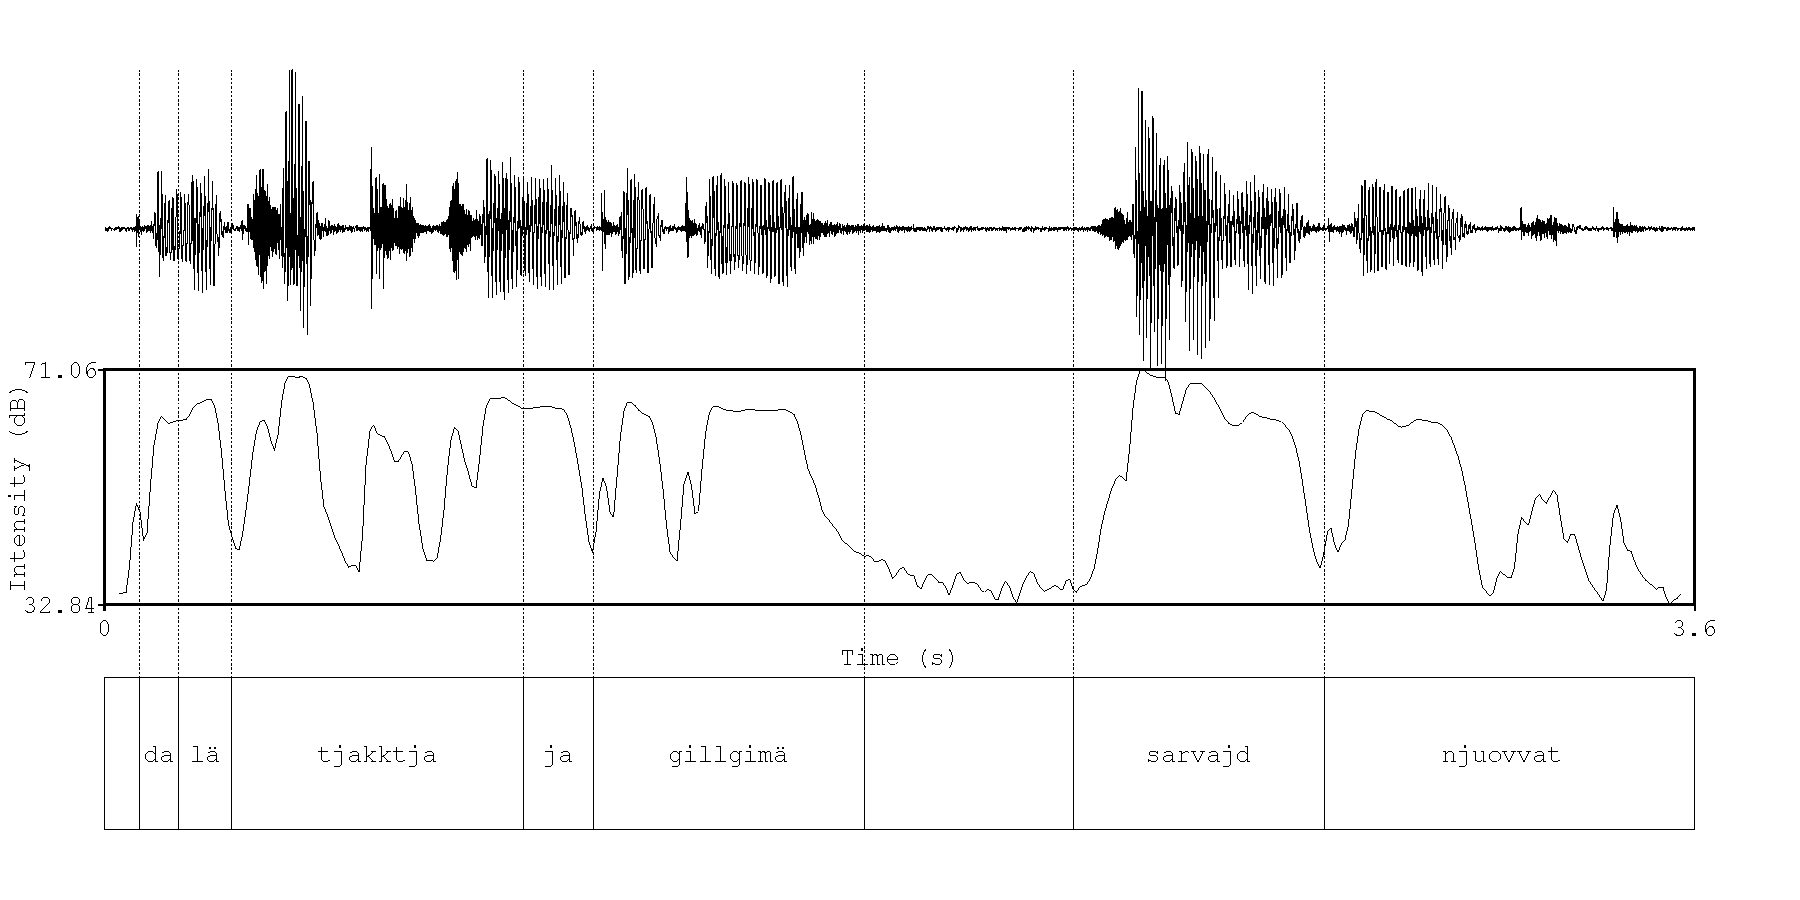
\includegraphics[width=.95\textwidth]{images/pit090826-003.pdf}}
\caption{Waveform and intensity trace illustrating the drop in intensity at the end of an utterance}\label{intonationGraphic}
\end{figure}
Here, the initial syllable nucleus of the first lexical item in the sentence 
\It{tjakttja} has an intensity of 69.7 dB, the other lexical items hover between 63.5 dB and 70.3 dB, while the final lexical item \It{njuovvat} begins at 64 dB on the initial syllable nucleus, and drops abrubtly to 50 dB on the final syllable nucleus. 



\subsection{Utterance-final weakening}\index{prosody!weakening}\label{utteranceFinalDevoicing}
The final two or three syllables of a declarative utterance in \PS\ can be weakened as a way to mark the end of an utterance.\footnote{\It{Arjeplogsmål}, the local Swedish dialect, features a similar phenomenon.} 
This weakening is typically is realized by completely devoicing the final one, two or three syllables, often to the point that these are whispered. Alternatively, this can be realized as creaky voice instead of voicelessness. For instance, in the example utterance transcribed in \REF{utteranceFinalDevoicing1} and depicted in the waveform in Figure \vref{utteranceFinalDevoicingGraphic}, devoicing occurs in the final lexical word \It{giesev} ‘summer’, which contains the last two syllables of the utterance. 
The lack of energy in the wave form corresponding to \It{giesev} shows clearly that the word is weakened significantly compared to the rest of the utterance. Note that even the vowels are completely devoiced.

\ea\label{utteranceFinalDevoicing1}%JW: not really good example because ’s’ is voiceless anyway, although the Vs are obviously devoiced - the point is that it’s nearly whispered, which is clearer in the wave-form
\glll	da’l adnam buorak, buorak giesev\\
	t-a=l at̚na-m pʊ͡ɔrakʰ pʊ͡ɔrak k\Bf{ɪ̥͡e̥se̥-v̥}\\
	\Sc{dem}-\Sc{3pl.nom}=be\BS\sc{3pl.prs} have-\sc{prf} good good summer-\sc{acc.sg}\\\nopagebreak
\Transl{they have had a good summer}{} \Corpus{090826}{012}
%\ex\label{utteranceFinalDevoicing1}
%\glll	dä dieda nubbe sábme diehta guk botsoj vuojdnuj\\
%	tɛ tɪ͡eta nupːe saːp̚me tɪ͡eʰta kukʰ poʦoj vʊ͡oj\Bf{j̥t̚n̥ɔ̥j̥}\\
%	then know\BS\sc{2sg.prs} other Saami\BS\sc{nom.sg} know\BS\sc{3sg.prs} how reindeer\BS\sc{nom.sg} look-\sc{3sg.pst}\\
%\Transl{then you know, the other Saami knows what the reindeer looked like}{} \Corpus{100405b.067}
\z
\begin{figure}
\fbox{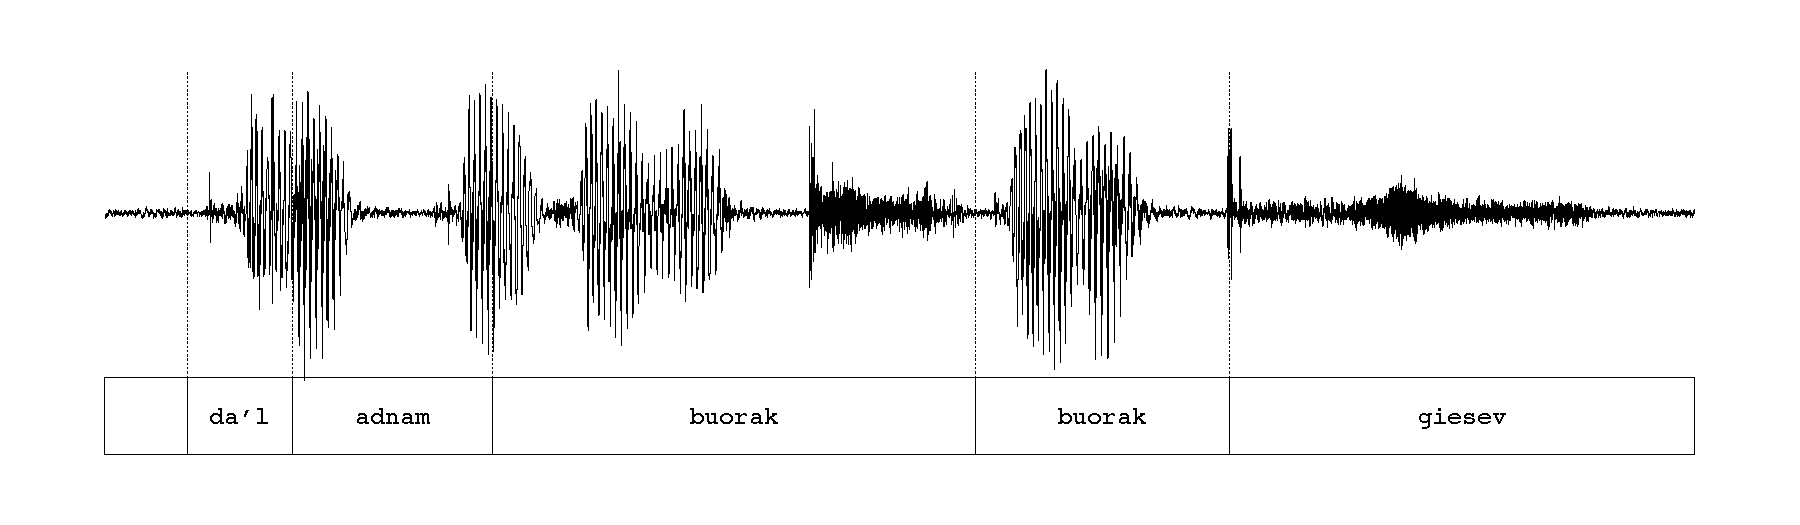
\includegraphics[width=.95\textwidth]{images/pit090826-012.pdf}}
\caption{Waveform illustrating utterance-final weakening}\label{utteranceFinalDevoicingGraphic}
\end{figure}

\korr{042}It is not clear what triggers this devoicing, and future study, particularly looking at the possibility of it being a turn marker in discourse, is needed.



%%%%%%%%%%%%%%%%%%%%%%%%%%%%%% S E G M E N T A L   P H O N O L O G Y %%%%%%%%%%%%%%%%%%%%%%%%%%%%%
%%%%%%%%%%%%%%%%%%%%%%%%%%%%%% S E G M E N T A L   P H O N O L O G Y %%%%%%%%%%%%%%%%%%%%%%%%%%%%%
%%%%%%%%%%%%%%%%%%%%%%%%%%%%%% S E G M E N T A L   P H O N O L O G Y %%%%%%%%%%%%%%%%%%%%%%%%%%%%%
%%%%%%%%%%%%%%%%%%%%%%%%%%%%%% S E G M E N T A L   P H O N O L O G Y %%%%%%%%%%%%%%%%%%%%%%%%%%%%%
%%%%%%%%%%%%%%%%%%%%%%%%%%%%%% S E G M E N T A L   P H O N O L O G Y %%%%%%%%%%%%%%%%%%%%%%%%%%%%%
%%%%%%%%%%%%%%%%%%%%%%%%%%%%%% S E G M E N T A L   P H O N O L O G Y %%%%%%%%%%%%%%%%%%%%%%%%%%%%%
\chapter{Segmental phonology}\index{phonology!consonants}\index{phonology!vowels}\label{csANDvs}
\PS\ has 43 \korr{043}consonant phonemes and 9 vowel phonemes. In the present chapter, the first section (\REF{consonants}) deals with consonants phonemes, their allophonic variation, and consonant clusters. 
The following section (\REF{vowels}) covers vowel phonemes, their allophonic variation, and schwa-epenthesis. 

%\Red{Note that Section \ref{orthography} provides an overview of the working \PS\ orthography and how it relates to \PS\ phonology. While most of the discussion in this chapter on segmental phonology includes both phonemic and phonetic transcriptions, other chapters only feature the orthographic representation when phonology is not directly relevant. }%moved from intro to Ch. 2, now part of explaining examples in Ch. 1


\section{Consonants}\label{consonants}\index{consonants}\label{CphoneInventory}
The consonant phoneme inventory of Pite Saami can be found in Table \vref{Cphonemes}.  
There are plain and preaspirated phonemes for all plosive and affricate positions, and geminate and singleton pairs for all categories. 
Preaspirated, geminate and preaspirated geminate phonemes are restricted to the consonant center position. 
\begin{table}\centering
\caption[Consonant phoneme inventory]{Consonant phoneme inventory}\label{Cphonemes}
\resizebox{1\linewidth}{!} {
\begin{tabular}{r c c c c c c c}
& bilabial & labiodental & alveolar & post-alveolar & palatal & velar & glottal\\\cline{2-8}
\multirow{1}{*}{plosive} & \multicolumn{1}{|c|}{p ʰp pː ʰpː} &\multicolumn{1}{c|}{}& \multicolumn{1}{c|}{t ʰt tː ʰtː}&\multicolumn{1}{c|}{}&\multicolumn{1}{c|}{}&\multicolumn{1}{c|}{k ʰk kː ʰkː}&\multicolumn{1}{c|}{}\\\cline{2-8}%6
\multirow{1}{*}{affricate} &\multicolumn{1}{|c|}{}&\multicolumn{1}{c|}{}& \multicolumn{1}{c|}{ʦ ʰʦ ʦː ʰʦː} &\multicolumn{1}{c|}{ʧ ʰʧ ʧː ʰʧː}&\multicolumn{1}{c|}{}&\multicolumn{1}{c|}{}&\multicolumn{1}{c|}{}\\\cline{2-8}%4
\multirow{1}{*}{fricative} &\multicolumn{1}{|c|}{}& \multicolumn{1}{c|}{f fː v vː} &\multicolumn{1}{c|}{s sː}&\multicolumn{1}{c|}{ʃ ʃː}&\multicolumn{1}{c|}{}&\multicolumn{1}{c|}{}&\multicolumn{1}{c|}{h}\\\cline{2-8}%5
\multirow{1}{*}{nasal} &\multicolumn{1}{|c|}{m mː}&\multicolumn{1}{c|}{}&\multicolumn{1}{c|}{n nː} &\multicolumn{1}{c|}{}&\multicolumn{1}{c|}{ɲ ɲː} & \multicolumn{1}{|c|}{ŋ ŋː}&\multicolumn{1}{c|}{}\\\cline{2-8}%4
\multirow{1}{*}{trill}&\multicolumn{1}{|c|}{}&\multicolumn{1}{c|}{}&\multicolumn{1}{c|}{r rː}&\multicolumn{1}{c|}{}&\multicolumn{1}{c|}{}&\multicolumn{1}{c|}{}&\multicolumn{1}{c|}{}\\\cline{2-8}%1
\multirow{1}{*}{approx.}&\multicolumn{1}{|c|}{}&\multicolumn{1}{c|}{}&\multicolumn{1}{c|}{l lː}&\multicolumn{1}{c|}{}&\multicolumn{1}{c|}{j jː}&\multicolumn{1}{c|}{}&\multicolumn{1}{c|}{}\\\cline{2-8}%2
%%total: 22
\end{tabular}}
\end{table}

A description of the consonant phonemes and the distribution of their relevant allophones can be found in Section \ref{Callophones} for each mode of articulation. 
This is followed by a discussion of consonant clusters. 
For the sake of clarity, the term \It{postaspiration} will be used here to refer to what is normally simply referred to as \It{aspiration} in most linguistic literature; this decision also emphasizes the contrast to \It{preaspiration}, which is, in fact, more relevant for Pite Saami than postaspiration.


\subsection{Consonant phonemes and allophonic variations}\label{Callophones}\index{allophony}\index{consonants!allophony}
After a brief note on preaspiration in the following section (\ref{preaspiration}) and a discussion of gemination in Section \ref{geminateCs}, the consonant phonemes and their allophones are described in the remaining sections (\ref{Plosives} - \ref{oralSonorants}). They are grouped based on manner of articulation.


\subsubsection{Preaspiration}\label{preaspiration}\index{preaspiration}\noindent
In Pite Saami, preaspirated\footnote{As is hopefully evident from this discussion on preaspiration, the term ‘preaspiration’ is not entirely accurate from a phonetic-acoustic point of view since the acoustic correlate of this phenomenon is not actually aspiration in all cases. Nonetheless, there are several reasons to select this term: 1. in the majority of cases, the acoustic correlate is in fact preaspiration, 2. this phonemic phenomenon is often referred to as preaspiration in the literature on %\PS\ \korr{063}\citep{} 
other Saami languages (cf. e.g. \citet[54-55]{Sammallahti1998} %\citet[15,18]{Svonni2009} %Svonni2009 never defines preasp, just uses the word here and there
or \citet[57,67]{Feist2010}), and 3. preaspiration can be reconstructed for the half-long and long Proto-Saami plosive and affricate phonemes \citep[cf.][54]{Sammallahti1998} that became the current \PS\ preaspirated phonemes.} 
phonemes only occur in consonant center position. While preaspirated phonemes can be plosives or affricates, the phenomenon that goes along with them is essentially the same. %, and does not interact with the length of the phoneme it is part of. 
The period of aspiration, i.e., the voicelessness preceding the formation of the oral closure, is realized in different ways and depends on the preceding segment. If the preceding segment is a voiced continuant %\marginpar{check for better term than ‘continuant’?} %JW: continuant probably best; Marijn can’t think of a better term
consonant, then the final part of that segment is devoiced.\footnote{While a minimal contrast between a voiceless obstruent preceding a preaspirated consonant phoneme and a voiceless obstruent preceding a plain counterpart phoneme (e.g.: /st/ vs. /sʰt/) is theoretically possible, this cannot be detected because such a consonant cannot be devoiced as it is already voiceless (e.g.: /st/ \ARROW [st] and /sʰt/\ARROW [st]).} %\footnote{Obstruents never immediately precede /ʰp ʰt ʰk/.} 
When following a high front vowel /i/, preaspiration is realized as a voiceless palatal fricative [ç]. 
In all other cases, preaspiration is a voiceless glottal fricative [h]. This is summarized in Table \vref{preaspRealization}. %on page \pageref{preaspRealization}.
\begin{table}\centering
\caption{The phonetic realizations of preaspiration}\label{preaspRealization}
\begin{tabular}{| c | c | c |}\hline
\It{preceding segment}	& \It{realization of preaspiration}	&\It{example} \\\dline
voiced consonant		& end devoicing of voiced consonant &/mʰp/ \ARROW [mm̥p] \\%\hline
%\MC{2}{|c|}{ex.:	/...mʰp.../ \ARROW [...mm̥p...]}\\
\hline
high front vowel /i/		& voiceless palatal fricative [ç]	&/iʰp/ \ARROW [içp]\\%\hline
%\MC{2}{|c|}{ex.:	/...iʰp.../ \ARROW [...çp...]}\\
\hline
other vowels			& voiceless glottal fricative [h]	&/aʰp/ \ARROW [ahp]\\%\hline
%\MC{2}{|c|}{ex.:	/...aʰp.../ \ARROW [...ahp...]}\\
\hline
\end{tabular}
\end{table}


\subsubsection{Geminates}\label{geminateCs}
The occurrence of geminate consonants is restricted to the consonant center. %and indeed common 
As can be seen in Table \vref{Cphonemes}, only the glottal fricative /h/ does not have a comparable geminate phoneme. %In such cases, the two phonemes are realized together as a geminate. 
Geminate segments are realized with a longer overall duration than the corresponding singleton phonemes. This observation is based not only on speakers’ observations that such sounds are ‘longer’, but also on my own observations and analyses, including an acoustic-phonetic comparison of duration in geminate phonemes; cf.~Section \ref{plosiveDurationComparison} for a detailed comparison non-voiced plosive durations in the consonant center. 

For plosives and affricates, only one stop closure is formed, and the overall duration of the stop closure is longer than the duration of a corresponding single consonant. Some examples are provided in \REF{outside} through \REF{motherNOMSG}.
\PhonGlossWL{outside}{ta\Bf{pː}en}{ta\Bf{pː}en}{dabben}{\Sc{dem}\BS\Sc{iness.sg}}{3672}
\PhonGloss{ribbonNOMSG}{pa\Bf{tː}e}{pa\Bf{tː}e}{badde}{ribbon\BS\Sc{nom.sg}}{080701b}{.082}%{swadesh?}
\PhonGloss{windNOMSG1}{pɛ\Bf{kː}a}{pɛ\Bf{kː}a}{bägga}{wind\BS\Sc{nom.sg}}{080702b}{.067}%{swadesh?}
\PhonGlossWL{goINF}{vaː\Bf{ʦː}e-t}{va:\Bf{tːs}etʰ}{vádtset}{go-\Sc{inf}}{2049}
\PhonGlossWL{motherNOMSG}{ʧi\Bf{ʧː}e}{ʧi\Bf{tːʃ}e}{tjidtje}{mother\BS\Sc{nom.sg}}{3618}
Preaspirated plosive and affricate geminates also exist. %the first segment can be preaspirated, in which case, the period of preaspiration tends to be longer than for a single preaspirated segment not followed by the corresponding homorganic plosive or affricate. %Similarly, a preaspirated plosive or affricate can be followed by the corresponding plain plosive or affricate. 
In such cases, the duration of both the preaspiration phase and the following stop closure are longer than in the corresponding preaspirated single consonants. Some examples are found in \REF{cleverPREDSG} through \REF{fatherNOMSGb}.
\PhonGloss{cleverPREDSG}		{ʧɛ\Bf{ʰpː}e}		{ʧɛ\Bf{hpː}e}		{tjähppe}	{clever\BS\Sc{pred.sg}}		{090930b}{.077}
%\PhonGloss{milkingbowlNOMSG}	{naː\Bf{ʰpp}e}	{naː\Bf{hpː}e}	{náhppe}	{milking\_cup\BS\Sc{nom.sg}}	{080621}
\PhonGloss{canINF}				{maː\Bf{ʰtː}e-t}	{maː\Bf{htː}etʰ}	{máhttet}	{can-\Sc{inf}}			{080926}{.03m21s}
%\PhonGloss{wolfNOMSG}			{kum\Bf{ʰpp}e}	{kum\Bf{m̥pː}e}	{gummpe}	{wolf\BS\Sc{nom.sg}}		{0671}
%\PhonGloss{workINF}			{par\Bf{ʰkk}at}	{par\Bf{r̥kː}atʰ}	{barrgat}	{work-\Sc{inf}}			{101208.005}
\PhonGlossWL{turnAround3SGPST}{ma:\Bf{ʰʦː}a-j}{ma:\Bf{htːs}aj}{máhttsaj}{turn\_around-\Sc{3sg.pst}}{6613}
\PhonGlossWL{fatherNOMSGb}{a:\Bf{ʰʧː}e}{a:\Bf{htːʃ}e}{áhttje}{father\BS\Sc{nom.sg}}{0016}

For all other consonants, the overall duration of a geminate is longer than for the corresponding single consonant. Examples of such geminates are provided in \REF{areaNOMSG} through \REF{letINF}.
\PhonGlossWL{areaNOMSG}	{taː\Bf{fː}o}	{taː\Bf{fː}o}	{dáffo}	{area\BS\Sc{nom.sg}}		{2367}%
%\PhonGloss{rapids}	{raː\Bf{ff}e}	{raː\Bf{fː}e}	{ráffe}	{rapids\BS\Sc{nom.sg}}		{2713}%
\PhonGlossWL{peaceNOMSG}	{raː\Bf{vː}e}	{raː\Bf{vː}e}	{rávve}	{peace\BS\Sc{nom.sg}}		{1366}%
\PhonGlossWL{partNOMSG}	{ɔ\Bf{sː}e}	{ɔ\Bf{sː}e}	{åsse}	{part\BS\Sc{nom.sg}}	{2269}
\PhonGlossWL{horsetailNOMSG}	{ɔ\Bf{ʃː}e}	{ɔ\Bf{ʃː}e}	{åssje}	{horsetail\BS\Sc{nom.sg}}	{2270}
\PhonGloss{suck3SGPRS}{ɲa\Bf{mː}a}{ɲa\Bf{mː}a}{njamma}{suck\BS\Sc{3sg.prs}}{080701b}{.005a}
\PhonGlossWL{littleBitNOMSG}{pi\Bf{nː}a}{pi\Bf{nː}a}{binna}{little\_bit\BS\Sc{nom.sg}}{2446}
%\PhonGloss{eggNOMSG}{mɔ\Bf{nn}e}{mɔ\Bf{nː}e}{månne}{egg\BS\Sc{nom.sg}}{080621}
\PhonGloss{daughterInLawNOMSG}{ma\Bf{ɲː}e}{ma\Bf{ɲː}e}{mannje}{daughter\_in\_law\BS\Sc{nom.sg}}{080621}{.74m04s}
%\PhonGlossLongGloss{daughterInLawNOMSG}{ma\Bf{ɲː}e}{ma\Bf{ɲː}e}{mannje}{daughter\_in\_law\BS\Sc{nom.sg}}{080621}{.74m04s}
\PhonGloss{after}{ma\Bf{ŋː}el}{ma\Bf{ŋː}el}{maŋŋel}{after}{080924}{.529}
\PhonGlossWL{iceOverINF}{kɔ\Bf{rː}oti-t}{kɔ\Bf{rː}otɪtʰ}{gårrodit}{ice\_over-\Sc{inf}}{4693}
\PhonGlossWL{fireNOMSG}{tɔ\Bf{lː}ɔ}{tɔ\Bf{lː}ɔ}{dållå}{fire\BS\Sc{nom.sg}}{0421}%KORRECTED from NOM:PL to SG -- 18.09.2013
\PhonGlossWL{letINF}{paː\Bf{jː}a-t}{paː\Bf{jː}atʰ}{bájjat}{let-\Sc{inf}}{3439}

Due mostly to the nature of morphophonemic stem alternations, there are numerous minimal pairs differing only in the presence of a singleton versus a geminate consonant; \korr{044}cf. Section \ref{Cgrad} on consonant gradation for examples. %, and the series of two identical segments has often been treated as a phonemic geminates or as morphologically triggered gemination in the literature on both \PS\ and other Saami languages with similar phenomena (cf. \cite{Lehtiranta1992}:46-47; \cite{Sammallahti1998}:46-50; ). 

It is also possible to have geminate fricative or sonorant phonemes, as described above, followed by a plosive of affricate phoneme, as illustrated by the examples in \REF{tableNOMSG} through \REF{tightPREDSG}.
\PhonGlossWL{tableNOMSG}	{pɛ\Bf{vː}te}	{pɛ\Bf{vː}te}	{bävvde}	{table\BS\Sc{nom.sg}}		{0289}%
\PhonGlossWL{rapidsNOMSG}	{lu\Bf{sː}pe}	{lu\Bf{sː}pe}	{lusspe}	{rapids\BS\Sc{nom.sg}}		{1077}%
\PhonGlossWL{shall3SGPRS}	{ka\Bf{lː}ka}	{ka\Bf{lː}ka}	{gallga}	{will\BS\Sc{3sg.prs}}		{6626}%
\PhonGlossWL{tightPREDSG}	{kaː\Bf{rː}ʰʧe}	{kaː\Bf{rr̥}ʰʧe}	{gárrtje}	{tight\BS\Sc{pred.sg}}		{0554}%

A series of two identical consonant phonemes can arise at the internal stem boundary of a compound. In such cases, the resulting duration can be longer than for a single plosive, but is not necessarily so, as the two phonemes are often realized as a singleton, as in \REF{cervicalVertebraeNOMSG}.
\PhonGlossWL{cervicalVertebraeNOMSG}{ʧepo\Bf{t}\PLUS\Bf{t}a:k:te}{ʧi͡epo\Bf{t}a:kʰte}{tjiebotdákkte\footnotemark}{cervical\_vertebra\BS\Sc{nom.sg}}{3771}
%\PhonGlossLong{cervicalVertebraeNOMSG}{ʧepo\Bf{t}\PLUS\Bf{t}a:k:te}{ʧi͡epo\Bf{t}a:kʰte}{tjiebotdákkte\footnotemark}{cervical\_vertebra\BS\Sc{nom.sg}}{}{3771}
\footnotetext{The word \It{tjiebotdákkte} literally means ‘throat-bone’, cf. \It{tjiebot} ‘throat’ and \It{dákkte} ‘bone’.}
Due to the morpheme boundary separating such segments, it is clear that this is not a case of geminate phonemes, even if the realization may resemble that of a geminate. 


\subsubsection{Plosives}\label{Plosives}\index{consonants!plosives}%%%%%%%% PLOSIVES %%%%%%%%%%%%%%%
The plosive series in Pite Saami consists of the phonemes and their phonetic realizations shown in Figure \vref{PlosivePhonemes}. The distribution of the allophones will be discussed here. As all three relevant places of articulation behave in much the same way, the various manners of articulation for each place will be treated together.
\begin{figure}\begin{center}
\begin{tabular}{c c l}
/p/ &:& [p] [pʰ] [p̚\,] \\ %should be written with <b>
/pː/ &:& [pː] \\ %should be written with <bb>
/ʰp/ &:& [ʰp] \\ %should be written with <hp>
/ʰpː/ &:& [ʰpː] \\ %should be written with <hpp>
%/b/ &:& [b] \\ %only loans (?)
/t/ &:& [t] [tʰ] [t̚\,] \\%unreleased even before palatal (see butter.sg.nom)! probably just +CORONAL
/tː/ &:& [tː] \\
/ʰt/ &:& [ʰt] \\
/ʰtː/ &:& [ʰtː] \\
%/d/ &:& [d] \\ %only loans (?)
/k/ &:& [k] [kʰ] [k̚\,] \\
/kː/ &:& [kː] \\
/ʰk/ &:& [ʰk] \\
/ʰkː/ &:& [ʰkː] \\
%/g/ &:& [g] \\ %only loans (?)
\end{tabular}
\end{center}
\caption{Plosive and affricate phonemes and their realizations}\label{PlosivePhonemes}
\end{figure}


\paragraph{Voiceless singleton plosives /p t k/}\label{ptk}
The segments /p t k/ are bilabial, alveolar and velar (respectively) voiceless singleton plosive phonemes. %With the exception of their individual places of articulation, they essentially exhibit the same behavior and will be described together here. %JW: redundant, see previous paragraph
The voiceless singleton plosives can occur in all prosodic consonant positions and are subject to allophonic variation, depending on the prosodic environment. In syllable-onset position%word-initial position and intervocalically
, a plain (unaspirated) voiceless plosive [p\,t\,k] is produced, as seen in examples \REF{dogNOMSG} through \REF{goodADV1}. %\footnote{In these and the examples in the following sections on other consonant and vowel phonemes, the underlying phonological representation, the phonetic form, the orthographic form, the gloss, and the source of the phonetic form are listed for each instance and in that order. The relevant phones and phonemes are in bold face.}
\PhonGloss{dogNOMSG}{\Bf{p}ena}{\Bf{p}i͡ena}{bena}{dog\BS\Sc{nom.sg}}{090926}{.057}
\PhonGloss{wish3DUPRS}{saːvːa-\Bf{p}a}{saːʋːa\Bf{p}aʰ}{sávvabah}{wish-\Sc{3du.prs}}{100323a}{.060}
\PhonGloss{2SGNOM}{\Bf{t}ɔj}{\Bf{t}ɔj}{dåj}{\Sc{2sg.nom}}{100323a}{.014}
\PhonGloss{cheeseNOMPL}{vos\Bf{t}a}{ʋu͡ɔs\Bf{t}a}{vuosta}{cheese\BS\Sc{nom.pl}}{080917c}{.09m47s}
\PhonGloss{widePREDSG}{\Bf{k}op\Bf{t}ok}{\Bf{k}opʰ\Bf{t}okʰ}{gåbdåk}{wide\BS\Sc{pred.sg}}{091001}{.035}
\PhonGloss{drink1SGPRS}{ju\Bf{k}a-v}{jʊ\Bf{k}ɑʋ}{jugav}{drink-\Sc{1sg.prs}}{100323a}{.115}
\PhonGloss{goodADV1}{\Bf{p}ora-\Bf{k}it}{\Bf{p}u͡ora\Bf{k}ɪtʰ}{buoragit}{good-\Sc{adv}}{100323a}{.213}
%\PhonGloss{queenNOMSG}{\Bf{t}rotnək}{\Bf{t}rot̚nɘkʰ}{drodnik\footnotemark}{queen.\Sc{nom.sg}}{missing}
%\footnotetext{from Sw. \It{drottning}}
%\PhonGloss{icecreamNOMSG}{\Bf{k}laːsːa}{\Bf{k}laːsːa}{glássa\footnotemark}{ice\_cream.\Sc{nom.sg}}{missing}
%\footnotetext{from Sw. \It{glass} (<French \It{glace})}

The plain voiceless singleton pronunciations [p\,t\,k] %\marginpar{mention that {[k]} is farther back in velar position (sounds almost uvular) than in English/German/Swedish?} 
are also found in consonant clusters in word-onset position, an environment usually found in recent and older loan words from (North) Germanic, as in examples \REF{queenNOMSG} and \REF{icecreamNOMSG}. %
%\PhonGloss{queenNOMSG}{\Bf{t}rotnik}{\Bf{t}rot̚nikʰ}{drodnik}{queen\BS\Sc{nom.sg}}{missing}%\footnotetext{from Sw. \It{drottning}.}
%\PhonGloss{icecreamNOMSG}{\Bf{k}laːsːa}{\Bf{k}laːsːa}{glássa}{ice\_cream\BS\Sc{nom.sg}}{missing}%\footnotetext{from Sw. \It{glass} (<French \It{glace}).}
\PhonGlossWL{queenNOMSG}{\Bf{t}rotnik}{\Bf{t}rot̚nikʰ}{drodnik\footnotemark}{queen\BS\Sc{nom.sg}}{0377}\footnotetext{from Sw. \It{drottning}.}
\PhonGlossWL{icecreamNOMSG}{\Bf{k}laːsːa}{\Bf{k}laːsːa}{glássa\footnotemark}{ice\_cream\BS\Sc{nom.sg}}{0529}\footnotetext{from Sw. \It{glass} (<French \It{glace}).}

The voiceless singleton plosives phonemes are postaspirated word-finally\footnote{Note, however, that speakers from the northern parts of \PS\ territory tend to voice the voiceless plosives phonemes as [b d g] in word-final position.} 
as [pʰ\,tʰ\,kʰ], as in examples \REF{be1PLPRS} through \REF{alonePRED}, as well as when preceding a non-homor\-ga\-nic plosive or affricate, as in examples \REF{alonePRED} through \REF{whoopingCoughNOMSG}. This is also the case across an internal compound boundary, as in \REF{whoopingCoughNOMSG}.\footnote{The word \It{båktjanitgåssås} in \REF{whoopingCoughNOMSG} refers to the whooping cough, and is a compound composed of \It{båktjanit} ‘to suffocate’ and \It{gåssås} ‘cough’.}
 %\marginpar{check if this is true at internal border of compounds or before nonhomorganic nasal? also check grade of ex. \REF{hairNOMPL} and \REF{marshNOMSG} - maybe this is true for all phonemic lengths!}%maybe also at the internal word-border of a compound (but what are the criteria for compounds then?); maybe also before a nonhomorganic nasal?
\PhonGloss{be1PLPRS}{orːo-\Bf{p}}{orːo\Bf{pʰ}}{årrop}{be-\Sc{1pl.prs}}{100323a}{.158}
\PhonGloss{goodADV2}{pora-ki\Bf{t}}{pʊ͡ɔrakɪ\Bf{tʰ}}{buoragit}{good-\Sc{adv}}{100323a}{.213}
\PhonGloss{alonePRED}{i\Bf{k}to\Bf{k}}{i\Bf{kʰ}to\Bf{kʰ}}{iktuk}{alone}{100323a}{.169}
\PhonGloss{hairNOMPL}{vo\Bf{p}ta}{ʋu͡o\Bf{pʰ}ta}{vuopta}{hair\BS\Sc{nom.pl}}{080701b}{.092}%check if this is grade I
%\PhonGloss{marshNOMSG}{kɔ\Bf{tː}kɔ}{kɔ\Bf{tʰ}kːɔ}{gåttkå}{marsh\BS\Sc{nom.sg}}{}{0762}%check if this is grade I
%\PhonGlossLong{1}{2}{3}{4}{5}{6}
\PhonGlossWL{whoopingCoughNOMSG}{pɔ\Bf{kʧ}ani\Bf{t}\PLUS\Bf{k}ɔs:ɔs}{pɔ\Bf{kʰʧ}ani\Bf{tʰk}ɔs:ɔs}{båktjanitgåssås}{whooping\_cough\BS\Sc{nom.sg}}{5993}
%\PhonGlossLong{whoopingCoughNOMSG}{pɔ\Bf{kʧ}ani\Bf{t}\PLUS\Bf{k}ɔs:ɔs}{pɔ\Bf{kʰʧ}ani\Bf{tʰk}ɔs:ɔs}{båktjanitgåssås\footnotemark}{whooping\_cough\BS\Sc{nom.sg}}{}{5993}
%\footnotetext{The word \It{båktjanitgåssås} refers to the whooping cough, and is a compound composed of \It{båktjanit} ‘to suffocate’ and \It{gåssås} ‘cough’.}

For all three plosive singleton phonemes, the closure is not released when a homorganic consonant %sonorant 
follows; they are then realized as [p̚ t̚ k̚]. Word-internally, this situation is only found in the consonant center and with a homorganic sonorant, as shown in examples \REF{heartNOMSG1} through \REF{butterNOMSG}. 
\PhonGloss{heartNOMSG1}{vaːj\Bf{p}mo}{ʋaːj\Bf{p̚}mo}{vájbmo}{heart\BS\Sc{nom.sg}}{080701b}{.115}
\PhonGloss{have2DUIMP}%different example here for unreleased alveolar voiceless plosive before another alveolar C!
{e\Bf{t}ni-t}{e\Bf{t̚}nɪtʰ}{ednit}{have-\Sc{2du.imp}}{100323a}{.251}
\PhonGloss{iceNOMSG}{je\Bf{k}ŋa}{je\Bf{k̚}ŋa}{jegŋa}{ice\BS\Sc{nom.sg}}{080702b}{.070}
\PhonGloss{butterNOMSG}{vo\Bf{t}ja}{vʊ͡ɔ\Bf{t̚}ja}{vuodja}{butter\BS\Sc{nom.sg}}{080926}{.01m15s} %Check this transcription!
%\PhonGloss{be3PLPSTa}{li\Bf{t}jin}{li\Bf{t̚}jɪn}{lidjen}{be-\Sc{3pl.pst}}{081011.049}%JW: decided this example isn’t necessary, plus it’s a big weird b/c it’s listed as lijjin in the worlist
%\PhonGlossLong{cervicalVertebraeNOMSG}{ʧepo\Bf{t}\PLUS\Bf{t}a:k:te}{ʧi͡epo\Bf{t}a:kʰte}{tjiebotdákkte\footnotemark}{cervical\_vertebra\BS\Sc{nom.sg}}{3771}
%\footnotetext{\It{tjiebotdákkte} is a cervical vertebra, literally \It{tjiebot} ‘throat’ and \It{dákkte} ‘bone’.}


\paragraph{Voiceless geminate plosives /pː tː kː/}
The segments /pː tː kː/ are bilabial, alveolar and velar (respectively) geminate plosive phonemes. They are very restricted in their distribution as they only occur in the consonant center\footnote{Cf. \ref{CCent} for a description of the \It{consonant center}\index{consonant center}.} % in the literature on Saami languages, but this refers to morphophonological status, which I try to avoid here in this purely phonological description. One could also refer to this position in terms of feet; then, Pite Saami would have trochaic feet counting from the left, in which case the geminate plosive phonemes only occur foot-internally.}
and never occur word-initially or word-finally. %In speech, the oral closure of these phonemes tends to have a duration of between 200 and 300 milliseconds.\marginpar{does this need more solid statistical evidence?}
Examples for the geminate plosive phonemes can be found in examples \REF{there} through \REF{bayNOMSG1}.
\PhonGlossWL{there}{to\Bf{pː}en}{to\Bf{pː}en}{dobben}{yonder}{3581}
\PhonGloss{ribbonNOMSGb}{pa\Bf{tː}e}{pa\Bf{tː}e}{badde}{ribbon\BS\Sc{nom.sg}}{090930a}{.215}
\PhonGloss{windNOMSG1b}{pɛ\Bf{kː}a}{pɛ\Bf{kː}a}{bägga}{wind\BS\Sc{nom.sg}}{080621}{.77m27s}
\PhonGloss{bayNOMSG1}{lu͡a\Bf{kː}ta}{lʊ͡a\Bf{kː}ta}{luakkta}{bay\BS\Sc{nom.sg}}{080917c}{.03m51s}

%%%%These are examples for /ʰp ʰt ʰk/!!!
%\begin{exe}
%\PhonGloss{milkingbowlNOMPL}%not relevant for /pː/!
%\begin{tabular}{p{2cm} p{2cm} p{1.5cm} p{4cm} l}
%/naː\Bf{ʰp}e}{naː\Bf{ʰp}ɘ}{náhpe} &'milking\_cup-\Sc{nom.pl}}{080621}
%\end{tabular}
%\PhonGloss{want3SGPRS}
%\begin{tabular}{p{2cm} p{2cm} p{1.5cm} p{4cm} l}
%[si\Bf{ʰt}a}{si\Bf{tː}a}{sihta} &'want.\Sc{3sg.prs}}{080926}
%\end{tabular}
%\PhonGloss{drinkINF}
%\begin{tabular}{p{2cm} p{2cm} p{1.5cm} p{4cm} l}
%[ju\Bf{ʰk}atʰ}{ju\Bf{kː}at}{juhgat} &'drink-\Sc{inf}}{100323a.114}
%\end{tabular}
%\end{exe}


\paragraph{Preaspirated singleton plosives /ʰp ʰt ʰk/}
%\paragraph[Preaspirated singleton plosives \\/ʰp ʰt ʰk/]{Preaspirated singleton plosives /ʰp ʰt ʰk/}
The segments \mbox{/ʰp ʰt ʰk/} are preaspirated bilabial, alveolar and velar (respectively) singleton plosive phonemes. They are only licensed as the final consonant segment in the consonant center. % or onset of even syllables. %Their period of stop closure in speech is around 150 msec\marginpar{this needs more evidence, very impressionistic length}. 
Examples can be found in \REF{milkingbowlNOMPL} through \REF{thankACCSG}.
\PhonGloss{milkingbowlNOMPL}	{naː\Bf{ʰp}e}		{naː\Bf{hp}e}	{náhpe}	{milking\_cup\BS\Sc{nom.pl}}	{080621}{.55m16s}
\PhonGloss{houseNOMSGb}		{tɔ\Bf{ʰp}e}		{tɔ\Bf{hp}e}		{dåhpe}	{house\BS\Sc{nom.sg}}		{100310b}{.083}
\PhonGloss{towardsNorth}		{nurː\Bf{ʰt}as}	{nur\Bf{r̥t}as}	{nurrtas}	{towards\_the\_north}		{081011}{.177}
\PhonGlossWL{louseNOMSG}		{ti\Bf{ʰk}e}		{ti\Bf{çk}e}		{dihke}	{louse\BS\Sc{nom.sg}}		{2359}
\PhonGloss{thankACCSG}		{kij\Bf{ʰt}o-v}		{kij\Bf{j̥t}oʋ}		{gijtov}	{thank-\Sc{acc.sg}}		{080621}{.11m45s}

\paragraph{Preaspirated geminate plosives /ʰpː ʰtː ʰkː/}
%\paragraph[Preaspirated geminate plosives \\/ʰpː ʰtː ʰkː/]{Preaspirated geminate plosives /ʰpː ʰtː ʰkː/}
The segments \mbox{/ʰpː ʰtː ʰkː/} are preaspirated bilabial, alveolar and velar (respectively) geminate plosive phonemes. 
They are only licensed in the consonant center. %The period of stop closure is around 300 msec\marginpar{this needs more evidence, very impressionistic length}. Thus, it is indeed the length of the stop closure which is in contrast to the preaspirated singleton plosive phonemes. 
Examples can be found in \REF{cleverPREDSGb} through \REF{workINF}.
\PhonGloss{cleverPREDSGb}		{ʧɛ\Bf{ʰpː}e}		{ʧɛ\Bf{hpː}e}		{tjähppe}	{clever\BS\Sc{pred.sg}}		{090930b}{.077}
\PhonGloss{milkingbowlNOMSGb}	{naː\Bf{ʰpː}e}	{naː\Bf{hpː}e}	{náhppe}	{milking\_cup\BS\Sc{nom.sg}}	{080621}{.54m38s}
\PhonGloss{canINFb}			{maː\Bf{ʰtː}e-t}	{maː\Bf{htː}etʰ}	{máhttet}	{can-\Sc{inf}}			{080926}{.03m21s}
\PhonGlossWL{wolfNOMSG}			{kum\Bf{ʰpː}e}	{kum\Bf{m̥pː}e}	{gummpe}	{wolf\BS\Sc{nom.sg}}		{0671}
\PhonGloss{workINF}			{par\Bf{ʰkː}a-t}	{par\Bf{r̥kː}atʰ}	{barrgat}	{work-\Sc{inf}}			{101208}{.005}


\paragraph[Non-voiced plosive durations in the consonant center]{Comparison of non-voiced plosive durations in the consonant center}\label{plosiveDurationComparison}
While a thorough study of length phenomena in \PS\ is beyond the scope of the current study, it is worth noting the actual duration which the various plosive phonemes are realized with in the consonant center. %\footnote{The consonant center is the only position in which all plosive and affricate phonemes occur.}%JW: footnote not relevant!
Specifically, %\marginpar{add praat illustrations for these, at the latest for the final/print version} %JW: not worth it, wouldn’t really show much anyway, durations sufficient!
a plain geminate plosive and a singleton preaspirated plosive have approximately the same duration for the period of stop closure (around 300ms), and are at least 100ms longer than plain singleton plosives and 100ms shorter than a preaspirated geminate plosive. In this respect, plain geminate plosives and preaspirated singleton phonemes seem to group together concerning stop closure duration. 
%, plain singletons are significantly shorter than preaspirated singletons, and plain geminates are significantly shorter than preaspirated geminates. 
Table \vref{stopClosureComparision} %on page \pageref{stopClosureComparision} 
shows some (near) minimal sets and duration measurements as a comparison. However, this alignment seems to be irrelevant phonologically. 

\begin{table}\centering
\caption[Comparison of stop closure durations]{Minimal sets or near minimal sets for comparison of stop closure durations (in milliseconds) for plain and preaspirated singletons and geminates}\label{stopClosureComparision}
\resizebox{\columnwidth}{!}{%
\begin{tabular}{|c | c | c | c | c |}\cline{2-5}%\hline
\MC{1}{c|}{}	&\It{plain single}		& \It{plain geminate} 		& preasp. single			& preasp. geminate\\%\dline%\multirow{2}{*}{\It{preasp. geminate}\\
\MC{1}{c|}{}	&/p/					& /pː/					& /ʰp/					& /ʰpː/ \\\cline{2-5}
\MC{1}{c|}{}	&145-150ms			&320-340ms			&280-340ms				&460-490ms\\\cline{2-5}%\hline
\MC{1}{c|}{}	&\It{short}				&\MC{2}{c|}{\It{medium}}							&\It{long}	\\\hline
\MR{4}{*}{\begin{sideways}\It{set 1}\end{sideways}}	
			&tɔ\Bf{p}e			& tu\Bf{pː}en		& tɔ\Bf{ʰp}e				& tɔ\Bf{ʰpː}o\\
%			&tɔ.\Bf{p}e			& tu\Bf{p.p}en		& tɔ\Bf{ʰ.p}e				& tɔ\Bf{ʰp.p}o\\%JW: here with syllable boundaries!
			&150ms				&320ms				& 340ms					&490ms\\
			&\It{house\BS\Sc{gen.sg}}&\It{outside}			&\It{house\BS\Sc{nom.sg}}	&\It{sheath\BS\Sc{nom.sg}}\\
			&\hyperlink{pit100310b}{\small[pit100310b]}		& \small[3581]	&\hyperlink{pit100310b}{\small[pit100310b]}			& \small[3627]\\\hline
\MR{4}{*}{\begin{sideways}\It{set 2}\end{sideways}}
			&naː\Bf{p}erti-t		&nu\Bf{pː}e			& naː\Bf{ʰp}e			& naː\Bf{ʰpː}e\\
%			&naː\Bf{.p}er.ti-t		&nu\Bf{p.p}e			& naː\Bf{ʰ.p}e			& naː\Bf{ʰp.p}e\\%JW: here with syllable boundaries!
			&145ms				&340ms				&280ms					&460ms\\
			&\It{drill-\Sc{inf}}		&\It{other}				&\It{milking\_bowl\BS\Sc{nom.pl}}&\It{milking\_bowl\BS\Sc{nom.sg}} \\
			&\small[3378]	&\small[1317]	&\hyperlink{pit080917a}{\small[pit080917a]}		&\hyperlink{pit080917a}{\small[pit080917a]} \\\hline%\cline{2-5}
%			&145-150ms			&\MC{2}{c||}{280-340ms}							&460-490ms\\\hline
%\MC{1}{c|}{}	&\It{short				&\MC{2}{c|}{\It{medium}							&\It{long	\\\cline{2-5}
\end{tabular}}
\end{table}


%%%%%%%% AFFRICATES %%%%%%%%%%%%%%%
%%%%%%%% AFFRICATES %%%%%%%%%%%%%%%
\subsubsection{Affricates}\label{Affricates}\index{consonants!affricates}
The affricate series in Pite Saami consists of the phones and their phonetic realizations shown in Figure \vref{AffricatePhonemes}. As affricates, they begin as a plosive stop, which is then released into a sibilant fricative. %They very closely resemble the plosive series, as discussed above in Section \ref{Plosives}, in their phonotactic restrictions. %\marginpar{or just include these with the regular plosives?}
These are described below.
\begin{figure}\centering
\begin{tabular}{c c l}
/ʦ/ &:& [ʦ] \\ %should be written as <ts>
/ʦː/ &:& [tːs] \\ %should be written as <hts>
/ʰʦ/ &:& [ʰʦ] \\ %should be written as <hhts>
/ʰʦː/ &:& [ʰtːs] \\ %should be written as <hhts>
/ʧ/ &:& [ʧ] \\ %should be written as <ts>
/ʧː/ &:& [tːʃ] \\ %should be written as <hts>
/ʰʧ/ &:& [ʰʧ] \\ %should be written as <hhts>
/ʰʧː/ &:& [ʰtːʃ] \\ %should be written as <hhts>
\end{tabular}
\caption{Affricate phonemes and their phonetic realizations}\label{AffricatePhonemes}
\end{figure}

\paragraph{Plain singleton affricates /ʦ ʧ/}\label{tstj}
The segments /ʦ ʧ/ are unvoiced alveolar and postalveolar (respectively) singleton affricate phonemes. Both can occur in syllable onset position. Examples can be found in \REF{peeINF} through \REF{wringINF}.
\PhonGlossWL{peeINF}{\Bf{ʦ}isːa-t}{\Bf{ʦ}isːatʰ}{tsissat}{pee-\Sc{inf}}{3700}
\PhonGlossWL{reindeerNOMSG}{pɔ\Bf{ʦ}oj}{pɔ\Bf{ʦ}oj}{båtsoj}{reindeer\BS\Sc{nom.sg}}{0263}
\PhonGlossWL{waterGENSG}{\Bf{ʧ}aː\Bf{ʦ}e-v}{\Bf{ʧ}aː\Bf{ʦ}ev}{tjátsev}{water-\Sc{gen.sg}}{1861}
\PhonGlossWL{wringINF}{pɔ\Bf{ʧ}esti-t}{pɔ\Bf{ʧ}estitʰ}{båtjestit}{wring-\Sc{inf}}{0262}%probably a derivation of båhtjet - ‘milk’!

The postalveolar affricate /ʧ/ can also occur in word-final\footnote{There is one particle \It{guts} with the alveolar affricate in final position, but it is not clear what this is or whether it is /ʦ/ or /tʦ/ in the consonant center (it is spelled inconsistently, as well). Noticeably, it is monosyllablic, and could be an abbreviated form of a typical bisyllabic word which has been lexicalized in its rapid-speech form, in which case it was historically in word-medial position.} % but the second syllable is lost in rapid speech in this particular phrase.} 
position, frequently as the diminutive suffix \It{-tj}, as in \REF{dogDIM}.
\PhonGlossWL{dogDIM}{petnaka-\Bf{ʧ}}{pet̚naka\Bf{ʧ}}{bednagatj}{dog-\Sc{dim}\BS\Sc{nom.sg}}{5717}

\paragraph{Plain geminate affricates /ʦː\,ʧː/}
The segments /ʦː\,ʧː/ are unvoiced alveolar and postalveolar (respectively) geminate affricate phonemes. As with all other geminates, the affricate geminates only occur in the consonant center. The duration of the stop closure is longer in geminate affricates compared to their singleton affricate counterparts, while the duration of the fricative element is not relevant.
Examples can be found in \REF{goINFb} and \REF{motherNOMSGb}.
\PhonGlossWL{goINFb}{vaː\Bf{ʦ:}e-t}{va:\Bf{tːs}etʰ}{vádtset}{go-\Sc{inf}}{2049}
\PhonGlossWL{motherNOMSGb}{ʧi\Bf{ʧ:}e}{ʧi\Bf{tːʃ}e}{tjidtje}{mother\BS\Sc{nom.sg}}{3618}

\paragraph{Preaspirated singleton affricates /ʰʦ ʰʧ/}
%\paragraph[Preaspirated singleton affricates \\/ʰʦ ʰʧ/]{Preaspirated singleton affricates /ʰʦ ʰʧ/}
The segments \mbox{/ʰʦ ʰʧ/} are preaspirated alveolar and postalveolar (respectively) singleton affricate phonemes. Just as with the preaspirated plosives, the preaspirated affricates only occur in the consonant center. Examples can be found in \REF{reindeerNOMPL} through \REF{henNOMSG}.
\PhonGloss{reindeerNOMPL}{pu\Bf{ʰʦ}u}{pu\Bf{hʦ}u}{buhtsu}{reindeer\BS\Sc{nom.pl}}{110413b}{.085}
%\PhonGloss{waterNOMSG}{ʧaː\Bf{ʰʦ}e}{ʧaː\Bf{hʦ}e}{tjáhtse}{water\BS\Sc{nom.sg}}{??}%JW: too many examples, removed this one
\PhonGlossWL{milkINF}{pɔ\Bf{ʰʧ}e-t}{pɔ\Bf{hʧ}etʰ}{båhtjet}{milk-\Sc{inf}}{0239}
\PhonGlossWL{henNOMSG}{vu͡anː\Bf{ʰʦ}a}{vʊ͡an\Bf{n̥ʦ}a}{vuanntsa}{hen\BS\Sc{nom.sg}}{2140}

\paragraph{Preaspirated geminate affricates /ʰʦː ʰʧː/}
%\paragraph[Preaspirated geminate affricates \\/ʰʦː ʰʧː/]{Preaspirated geminate affricates /ʰʦː ʰʧː/}
The segments \mbox{/ʰʦː ʰʧː/} are preaspirated alveolar and postalveolar (respectively) geminate affricate phonemes. 
Just as with the preaspirated geminate plosives, the preaspirated geminate affricates only occur in the consonant center. The duration of the preaspiration and stop closure is longer in geminate affricates compared to their singleton affricate counterparts, while the duration of the fricative element is not phonologically relevant. 
Examples can be found in \REF{turnAround3SGPSTb} and \REF{fatherNOMSG}.
\PhonGlossWL{turnAround3SGPSTb}{ma:\Bf{ʰʦ:}a-j}{ma:\Bf{htːs}aj}{máhttsaj}{turn\_around-\Sc{3sg.pst}}{6613}
\PhonGloss{fatherNOMSG}{a:\Bf{ʰʧ:}e}{a:\Bf{htːʃ}e}{áhttje}{father\BS\Sc{nom.sg}}{110415}{.19m16s}


%%%%%%%% FRICATIVES %%%%%%%%%%%%%%%
%%%%%%%% FRICATIVES %%%%%%%%%%%%%%%
%%%%%%%% FRICATIVES %%%%%%%%%%%%%%%
\subsubsection{Fricatives}\label{Fricatives}\index{consonants!fricatives}
The fricative series in Pite Saami consists of the phonemes and their phonetic realizations shown in Figure \vref{FricativePhonemes}. %Just as with the other consonants in Pite Saami, the fricative phonemes include singletons and geminates. %The distribution of the relevant allophones will be discussed here.
\begin{figure}\centering
\begin{tabular}{c c l}
/f/ &:& [f] \\ %should be written as <f>
/fː/ &:& [fː] \\ %should be written as <ff>
/v/ &:& [v] [vv̥] [ʋ] \\ %should be written as <v>
/vː/ &:& [vː] [vv̥ː] [ʋː] \\ %should be written as <vv>
/s/ &:& [s] \\ %should be written as <s>
/sː/ &:& [sː] \\ %should be written as <ss>
/ʃ/ &:& [ʃ] \\ %should be written as <sj>
/ʃː/ &:& [ʃː] \\ %should be written as <ssj>
/h/ &:& [h] \\ %should be written as <h>
\end{tabular}
\caption{Fricative phonemes and their realizations}\label{FricativePhonemes}
\end{figure}

\paragraph{Singleton fricative consonants /f v s ʃ h/}\label{fvssjh}
%\paragraph[Singleton fricative consonants \\/f v s ʃ h/]{Singleton fricative consonants /f v s ʃ h/}
The segments \mbox{/f v s ʃ h/} are singleton labiodental (unvoiced and voiced), alveolar, post-alveolar and glottal fricatives, all of which are attested in syllable onset and word-internal coda position. %and in the consonant center. 
Some examples are provided in \REF{areaELATSG} through \REF{evilNOMSG}.
%\PhonGloss{beautifulATTR}	{\Bf{f}aː\Bf{vː}ro}		{\Bf{f}aː\Bf{vː}ro}		{fávvro}	{beautiful\BS\Sc{attr}}		{}{0472}%JW: this -v- maybe not in bold because it’s in a CC?
\PhonGlossWL{areaELATSG}	{taː\Bf{f}o-st}		{taː\Bf{f}ostʰ}		{dáfost}	{area-\Sc{elat.sg}}		{6803}
\PhonGloss{sonInLawACCSG}	{\Bf{v}i\Bf{v}a-v}	{\Bf{v}i\Bf{v}ɑʋ}		{vivav}	{son\_in\_law-\Sc{acc.sg}}	{110415}{.08m08s}
\PhonGlossWL{speakINFb}		{\Bf{s}aːka\Bf{s}ti-t}	{\Bf{s}aːka\Bf{s}tɪtʰ}	{ságastit}	{speak-\Sc{inf}}		{1480}
\PhonGloss{summerINESSSG}	{ke\Bf{s}e-n}		{ki͡e\Bf{s}en}		{giesen}	{summer-\Sc{iness.sg}}	{100310b}{.019}
\PhonGlossWL{ugly}			{\Bf{ʃ}ulːo}			{\Bf{ʃ}ulːo}			{sjullo}	{ugly\Sc{}}		{1598}
\PhonGlossWL{think1SGPRS}	{u\Bf{ʃ}uta-v}		{u\Bf{ʃ}utɑʋ}		{usjudav}	{think-\Sc{1sg.prs}}		{6815}
\PhonGlossWL{sayINF}			{\Bf{h}ɔlːɔ-t}		{\Bf{h}ɔlːotʰ}		{hållåt}	{say-\Sc{inf}}	{0856}
\PhonGlossWL{evilNOMSG}		{pa\Bf{h}aː}		{pa\Bf{h}aː}		{bahá}	{evil\BS\Sc{nom.sg}}	{0101}

The phonemes /v s/ can also occur in word-final position, as in examples \REF{fordNOMSG} and \REF{bad}.%\marginpar{mention that -sj (-ʃ) is DIM for some speakers?}
\PhonGlossWL{fordNOMSG}	{kaːlaː-\Bf{v}}	{kaːlɑː\Bf{v}}	{gáláv}	{ford\BS\Sc{nom.sg}}	{4332}
%\PhonGloss{grandchildNOMSG}	{aːtjo\Bf{v}}	{aːt̚jo\Bf{v}}	{ádjov}	{grandchild\BS\Sc{nom.sg}}	{}{0005}
\PhonGlossWL{bad}		{nevre\Bf{s}}	{ni͡evre\Bf{s}}	{nievres}	{bad\Sc{}}	{5101}
%\PhonGloss{evilNOMSG}		{pa\Bf{h}aː}		{pa\Bf{h}aː}		{bahá}	{evil\BS\Sc{nom.sg}}	{0101}
For some speakers from the north-eastern parts of \PS\ territory, /ʃ/ is also possible word-finally because the diminutive suffix is sometimes \It{-ʃ} (instead of \It{-ʧ}); however there is not enough data in the corpus to determine when the diminutive suffix is /-ʃ/. 

Two of these phonemes require further explanation. First of all, the bilabial voiced fricative /v/ is often realized as a labio-dental approximant [ʋ] when following an open front vowel /a/ or /aː/, as illustrated by examples \REF{sonInLawACCSG} and \REF{think1SGPRS} above.\footnote{This fact is even evident in some Swedish place-name spellings which use the more open vowel-like spelling <au> instead of the fricative spelling <av>, such as in \It{Båtsjaur}, a small community near Arjeplog whose name is likely based on the (Pite) Saami words \It{båtsoj} 'reindeer' and \It{jávvre} 'lake’.} %EVIDENCE FOR THIS ETYMOLOGY?? 
In this case, the open front vowel is realized as a back vowel [ɑ]. 
Furthermore, /v/ is frequently realized as either [ʋ] or as a voiced labial-velar approximant [w] in word-initial position as well, particularly in the Pite Saami dialects along the Pite River to the north. However, the [ʋ] pronunciation seems to be in free variation with a fricative [v] sound. 
%Because careful pronunciations prefer [v] over [ʋ] and for the sake of symmetry in the phoneme inventory, I have chosen to represent this sound phonemically with /v/. 
This is illustrated by the example in \REF{cheeseNOMSG}.% and \ref{wish1SGPRS}.
\ea\label{cheeseNOMSG}
\begin{tabular}{p{18mm} x{22mm} l }%p{90pt}}
\multirow{2}{*}{/\Bf{v}u͡asːta/} &[\Bf{w}u͡asːta]\textasciitilde & \It{vuassta}		\\%&\hfill\hyperlink{110517b2}{\small[pit110517b2.038]}\\
					 &[\Bf{v}u͡asːta] 			& 'cheese\BS\Sc{nom.sg}'	\\%&\hfill\hyperlink{080917c}{\small[pit080917c.9m42s]}\\
\end{tabular}
\hfill\pbox{\textwidth}{\hfill\hyperlink{pit110517b2}{\small[pit110517b2.038]}\\\hfill\hyperlink{pit080917c}{\small[pit080917c.9m42s]}}
\z

Secondly, a glottal fricative [h] as the sole consonant in word-final position is possible, but it seems to be limited to certain morphological conditions in contemporary Pite Saami, and only realized by some speakers, and then inconsistently. 
%Because it is optional, it does not have phonological status in word-final position. %JW: removed after comment from UM  
However, some of the literature describing older stages of Pite Saami\footnote{Cf. the paradigms in \citet[150-159]{Lehtiranta1992} indicate that there is an \It{-h} suffix for \Sc{nom.pl}, \Sc{gen.sg}, \Sc{conneg} and \Sc{2sg.prs}, among others. Note that \citet{Lehtiranta1992} describes \PS\ up through 1950, but not after that. Also note that \citet[104;120]{Lagercrantz1926} claims that no suffixes exist in these morphosyntactic contexts.} indicates that at a previous stage of the language, a word-final /h/ was obligatory when it had morphological status%(cf. the morphological environments triggered by \Sc{2sg.prs} or \Sc{gen.sg}, among others)%\marginpar{Perhaps this refers too much to morphophonology - but except in the morphological environments mentioned, /h/ is never word-final and never optional; perhaps a better analysis would be to say that these suffixes are optional, and it has nothing to do with phonology.}
. Two examples for this variation can be seen in \REF{work2SGPRS} and \REF{fishDIMGENSG}.
\ea\label{work2SGPRS}
\begin{tabular}{p{18mm} x{22mm} l}
\multirow{2}{*}{/parka/}	&[parka]\textasciitilde	& \It{barga}			\\
					&[parka\Bf{h}] 			& ‘work\BS\Sc{conneg}’ 	\\
\end{tabular}
\hfill\pbox{\textwidth}{\hfill\hyperlink{pit101208}{\small[pit101208.032]}\\\hfill\hyperlink{pit101208}{\small[pit101208.029]}}
\z
\ea\label{fishDIMGENSG}
\begin{tabular}{p{18mm} x{23mm} l}
\multirow{2}{*}{/kolaː-ʧ-a/}	&[kʊ͡ɔlaːʧa]\textasciitilde	& \It{guolatja}			\\
					&[kʊ͡ɔlaːʧa\Bf{h}] 		& ‘fish-\Sc{dim}-\Sc{gen.sg}’ 	\\
\end{tabular}
\hfill\pbox{\textwidth}{\hfill\hyperlink{pit110413a}{\small[pit110413a.077]}\\\hfill\hyperlink{pit110413a}{\small[pit110413a.079]}}
\z



\paragraph{Geminate fricative consonant /fː\,vː\,sː\,ʃː/}
%\paragraph[Geminate fricative consonant \\/fː vː sː ʃː/]{Geminate fricative consonant /fː vː sː ʃː/}
The segments /fː\,vː\,sː\,ʃː/ are geminate labiodental (unvoiced and voiced), alveolar and post-alveolar fricatives. As with all geminate phonemes, these fricatives only occur in consonant center position. The unvoiced labiodental geminate /fː/ is rather uncommon and unique in this series in that it never occurs as part of a consonant cluster. Note that, unlike the singleton fricative series, there is no glottal geminate fricative phoneme /hː/. Some examples are provided in \REF{areaNOMSGb} through \REF{horsetailNOMSGb}.
\PhonGlossWL{areaNOMSGb}	{taː\Bf{fː}o}	{taː\Bf{fː}o}	{dáffo}	{area\BS\Sc{nom.sg}}		{2367}%
\PhonGlossWL{rapids}	{raː\Bf{fː}e}	{raː\Bf{fː}e}	{ráffe}	{rapids\BS\Sc{nom.sg}}		{2713}%
\PhonGlossWL{peaceNOMSGb}	{raː\Bf{vː}e}	{raː\Bf{vː}e}	{rávve}	{peace\BS\Sc{nom.sg}}		{1366}%
\PhonGlossWL{partNOMSGb}	{ɔ\Bf{sː}e}	{ɔ\Bf{sː}e}	{åsse}	{part\BS\Sc{nom.sg}}	{2269}
\PhonGlossWL{horsetailNOMSGb}	{ɔ\Bf{ʃː}e}	{ɔ\Bf{ʃː}e}	{åssje}	{horsetail\BS\Sc{nom.sg}}	{2270}


\paragraph{Fricatives and preaspiration}\label{fricativesAndPreaspiration}
When preceding a preaspirated segment, the voiced fricative phoneme /v/ becomes devoiced towards the end of its realization as [vv̥].\footnote{Cf. Section \ref{sonorantsAndPreaspiration} for essentially the same phenomenon in sonorant phonemes.} 
The near minimal pair illustrated by the examples in \REF{predatorNOMSG} and \REF{likeThis} shows a voiced fricative preceding a plain and a preaspirated plosive, respectively.
\PhonGlossWL{predatorNOMSG}	{naː\Bf{vːt}e}	{naː\Bf{vːt}e}	{návvde}	{predator\BS\Sc{nom.sg}}		{6042}%
\PhonGlossWL{likeThis}		{naː\Bf{vʰt}ɛ}	{naː\Bf{vv̥t}ɛ}	{návte}	{like this}		{1252}%
Evidence for a preaspirated segment following the other fricatives is impossible to ascertain due to their inherent voicelessness.



%%%%%%%% NASALS %%%%%%%%%%%%%%%
%%%%%%%% NASALS %%%%%%%%%%%%%%%
\subsubsection{Nasals}\label{Nasals}\index{consonants!nasals}%%%%%%%% NASALS %%%%%%%%%%%%%%%
The nasal series in Pite Saami consists of the phones and their phonetic realizations shown in Figure \vref{NasalPhonemes}. The distribution of the allophones will be discussed here; see Section \ref{sonorantsAndPreaspiration} specifically for the devoiced allophones. 
\begin{figure}\centering
\begin{tabular}{l c l}
/m/ &:& [m] [mm̥] \\ %should be written as <m>
/mː/ &:& [mː] [mm̥:] \\ %should be written as <mm>
/n/ &:& [n] [nn̥] \\ %should be written as <n>
/nː/ &:& [nː] [nn̥:]\\ %should be written as <nn>
/ɲ/ &:& [ɲ] [ɲɲ̥]\\ %should be written as <nj>
/ɲː/ &:& [ɲː] [ɲɲ̥:]\\ %should be written as <nnj> %does this really exist?
/ŋ/ &:& [ŋ] [ŋŋ̥]\\ %should be written as <ng>
/ŋː/ &:& [ŋː] [ŋŋ̥:]\\ %should be written as <nng>  %does this really exist?
\end{tabular}
\caption{Nasal phonemes and their realizations}\label{NasalPhonemes}
\end{figure}


\paragraph{Singleton nasal consonants /m n ɲ ŋ/}
The segments /m n ɲ ŋ/ are singleton bilabial, alveolar, palatal and velar (respectively) nasal consonant phonemes. 
They can be found in onset and coda positions, with the exception of the velar nasal, which cannot appear word-initially\footnote{A phonotactic restriction barring a phonemic velar nasal in word-initial position is a common trait for languages spoken in Europe and western Asia \citep[cf.][]{Anderson2008WALS}.} and is only attested once word-finally (shown in example \REF{sometimes}). Some examples for singleton nasal phonemes in various positions within words can be found in \REF{1SGNOM} through \REF{sometimes}. %\marginpar{unsure about ŋ in final position; ex. \ref{sometimes} from wordlist only - not from own data!}
\PhonGloss{1SGNOM}			{\Bf{m}o\Bf{n}}{\Bf{m}o\Bf{n}}{mån}	{\Sc{1sg.nom}}			{100323a}{.004}
\PhonGloss{reside1DUPST}		{ɔro-j\Bf{m}en}	{ɔroj\Bf{m}ɘn}	{årojmen}	{reside-\Sc{1du.pst}}		{100323a}{.181}
\PhonGloss{eatPRF}				{pɔrːo-\Bf{m}}	{pɔrːo\Bf{m}}	{bårrom}	{eat-\Sc{prf}}			{100323a}{.103}
\PhonGlossWL{glueINF}				{ɲi\Bf{m}ki-t}		{ɲɪ\Bf{m}kitʰ}	{njimgit}	{glue-\Sc{inf}}			{1287}
\PhonGloss{girlNOMSG}			{\Bf{n}ɛjːta}		{\Bf{n}ɛj̥ːta}		{näjjda}	{girl\BS\Sc{nom.sg}}		{110415}{.06m31s}
\PhonGloss{bearNOMSG}			{pɛrt\Bf{n}a}		{pɛr̥t̚\Bf{n}a}		{bärdna}	{bear\BS\Sc{nom.sg}}		{080926}{.01m19s}
\PhonGloss{breastNOMSG}		{\Bf{ɲ}iʰʧːe}		{\Bf{ɲ}iʰʧːe}		{njiddtje}	{breast\BS\Sc{nom.sg}}	{080701b}{.114}
\PhonGloss{daughterInLawNOMPL}	{ma\Bf{ɲ}e}		{ma\Bf{ɲ}e}		{manje}	{daughter\_in\_law\BS\Sc{nom.pl}}{080621}{.74m26s}
%\PhonGlossLongGloss{daughterInLawNOMPL}	{ma\Bf{ɲ}e}		{ma\Bf{ɲ}e}		{manje}	{daughter\_in\_law\BS\Sc{nom.pl}}{080621}{.74m26s}
\PhonGloss{namely}				{va\Bf{ɲ}}		{va\Bf{ɲ}}		{vanj}	{really}					{090702}{.035}
\PhonGloss{iceNOMSGb}			{jek\Bf{ŋ}a}		{ji͡ek\Bf{ŋ}a}		{jegŋa}	{ice\BS\Sc{nom.sg}}		{080702b}{.070}
\PhonGloss{sometimes}	{mudi\Bf{ŋ}}		{mudi\Bf{ŋ}}		{mudiŋ}	{sometimes}			{080708\_Session02}{.026}%
%\PhonGlossLongSource{sometimes}	{mudi\Bf{ŋ}}		{mudi\Bf{ŋ}}		{mudiŋ}	{sometimes}			{080708\_Session02}{.026}%

\paragraph{Geminate nasal consonants /mː nː ɲː ŋː/}
%\paragraph[Geminate nasal consonants \\/mː nː ɲː ŋː/]{Geminate nasal consonants /mː nː ɲː ŋː/}
The segments /mː nː ɲː ŋː/ are geminate bilabial, alveolar, palatal and velar (respectively) nasal consonant phonemes. 
As is the case for all other geminate phonemes, their distribution is restricted to the consonant center. Some examples with the geminate nasal phonemes can be found in \REF{suck3SGPRSb} through \REF{afterB}.
\PhonGloss{suck3SGPRSb}{ɲa\Bf{mː}a}{ɲa\Bf{mː}a}{njamma}{suck\BS\Sc{3sg.prs}}{080701b}{.01m38s}
\PhonGlossWL{littleBitNOMSGb}{pi\Bf{nː}a}{pi\Bf{nː}a}{binna}{little\_bit\BS\Sc{nom.sg}}{2446}
%\PhonGloss{eggNOMSG}{mɔ\Bf{nː}e}{mɔ\Bf{nː}e}{månne}{egg\BS\Sc{nom.sg}}{080621}
\PhonGloss{daughterInLawNOMSGb}{ma\Bf{ɲː}e}{ma\Bf{ɲː}e}{mannje}{daughter\_in\_law\BS\Sc{nom.sg}}{080621}{.74m05s}
%\PhonGlossLongGloss{daughterInLawNOMSGb}{ma\Bf{ɲː}e}{ma\Bf{ɲː}e}{mannje}{daughter\_in\_law\BS\Sc{nom.sg}}{080621}{.74m05s}
\PhonGloss{afterB}{ma\Bf{ŋː}el}{ma\Bf{ŋː}el}{maŋŋel}{after}{080924}{.529}



%%%%%%%% ORAL SONORANTS %%%%%%%%%%%%%%%
%%%%%%%% ORAL SONORANTS %%%%%%%%%%%%%%%
%%%%%%%% ORAL SONORANTS %%%%%%%%%%%%%%%
\subsubsection{Oral sonorants}\label{oralSonorants}\index{consonants!oral sonorants}\index{consonants!trills}\index{consonants!approximants}%\index{consonants!lateral approximants}
\PS\ has three oral sonorant phonemes; %they comprise three singleton-geminate pairs of oral sonorant phonemes. 
because their behavior is very similar, they will be described together in the rest of this section. 
Their phonetic realizations are shown in Figure \vref{oralSonorantPhonemes}. See Section \ref{sonorantsAndPreaspiration} specifically for the devoiced allophones.
\begin{figure}\centering
\begin{tabular}{c c l}
/r/ &:& [r] [rr̥] [ɾ]\\ %JW: removed [ɽ]
/rː/ &:& [rː] [rr̥ː] \\ %JW: removed [ɽ]
/l/ &:& [l] [ll̥]\\ %JW: removed [lʎ]
/lː/ &:& [lː] [ll̥ː]\\ %%JW: removed [ɬ] [lʎ]
%%/ʎ/? &:& [lj] \\ %should be written as <lj>
%%/ʎː/? &:& [lːj] \\ %should be written as <llj>
/j/ &:& [j] [jj̥] \\ %
/jː/ &:& [jː] [jj̥ː] \\ %
\end{tabular}
\caption{Oral sonorant phonemes and their realizations}\label{oralSonorantPhonemes}%\caption{Trill phonemes and their realizaitons.}\label{TrillPhonemes}
\end{figure}


%%%%%%%% TRILLS %%%%%%%%%%%%%%%
%%%%%%%% TRILLS %%%%%%%%%%%%%%%
%%%%%%%% TRILLS %%%%%%%%%%%%%%%
\paragraph{Singleton trill consonant /r/}
The segment /r/ is a singleton alveolar trill. It can occur in syllable onset and coda positions. %\Red{Some consonant clusters include /r/; see Section \ref{CClusters}.??} 
In rapid speech, it is often realized as an alveolar tap [ɾ], particularly intervocalically. Some examples are found in \REF{rainNOMSG} through \REF{snowdriftNOMSG}. It becomes devoiced [rr̥] towards the end of its realization when preceding a preaspirated phoneme. Word-finally, it is also optionally completely devoiced as [r̥].%However, only in word-internal position can it occur in a consonant cluster.
\PhonGlossWL{rainNOMSG}{\Bf{r}aːʃːo}{\Bf{r}aːʃːo}{rássjo}{rain\BS\Sc{nom.sg}}{1385}
%\PhonGloss{steep}{p\Bf{r}a\Bf{r}es}{p\Bf{r}a\Bf{r}es}{prares}{steep}{}{5789}
\PhonGlossWL{badB}{kɔ\Bf{r}ɔ}{kɔ\Bf{r}ɔ}{gårå}{bad}{0768}
\PhonGlossWL{wireCOMSG}{ɛ\Bf{r}ʰpo-jn}{ɛ\Bf{rr̥}pojn}{ärpojn}{wire-\sc{com.sg}}{6794}
\PhonGlossWL{snowdriftNOMSG}{felpa\Bf{r}}{felpa\Bf{r}}{fielbar}{snowdrift\BS\Sc{nom.sg}}{0473}

\paragraph{Geminate trill consonant /rː/}
The segment /rː/ is a geminate alveolar trill. It only occurs in the consonant center, as in \REF{iceOverINFb}.
\PhonGlossWL{iceOverINFb}{kɔ\Bf{rː}oti-t}{kɔ\Bf{rː}otɪtʰ}{gårrodit}{ice\_over-\Sc{INF}}{4693}


\paragraph{Singleton lateral approximant /l/}
The segment /l/ is a lateral approximant. It can occur in syllable onset and coda positions. 
Some examples are found in \REF{tenCARD} through \REF{jawNOMSG}. 
\PhonGlossWL{tenCARD}{\Bf{l}ɔkev}{\Bf{l}ɔkev}{lågev}{ten}{2313}%ten\BS\Sc{card}
\PhonGlossWL{getScared2SGPRS}{pa\Bf{l}a}{pa\Bf{l}a}{bala}{become\_scared\BS\Sc{2sg.prs}}{6332}
%\PhonGlossLongGloss{getScared2SGPRS}{pa\Bf{l}a}{pa\Bf{l}a}{bala}{become\_scared\BS\Sc{2sg.prs}}{}{6332}
%\PhonGloss{fireACCSG}{tɔ\Bf{l}ɔv}{tɔ\Bf{l}ɔv}{dålåv}{fire-\Sc{acc.sg}}{??}
\PhonGlossWL{shall1SGPRS}{ka\Bf{l}ka-v}{ka\Bf{l}kɑʋ}{galgav}{will-\Sc{1sg.prs}}{6627}
\PhonGlossWL{jawNOMSG}{ɔ\Bf{l}o\Bf{l}}{ɔ\Bf{l}o\Bf{l}}{ålol}{jaw\BS\Sc{nom.sg}}{2257}

\paragraph{Geminate lateral approximant /lː/}
The segment /lː/ is a singleton lateral approximant. It only occurs in the consonant center, as in \REF{fireNOMSGb}.
\PhonGlossWL{fireNOMSGb}{tɔ\Bf{lː}ɔ}{tɔ\Bf{lː}ɔ}{dållå}{fire\BS\Sc{nom.sg}}{0421}%KORRECTED from NOM:PL to SG -- 18.09.2013


\paragraph{Singleton central approximant /j/}
The segment /j/ is a central approximant phoneme. It can occur in syllable onset and coda positions. 
Some examples are found in \REF{iceNOMSGc} through \REF{shedILLSG}. 
\PhonGlossWL{iceNOMSGc}{\Bf{j}ekŋa}{\Bf{j}i͡ek̚ŋa}{jegŋa}{ice\BS\Sc{nom.sg}}{0922}%
\PhonGlossWL{waterSpringNOMSG}{aː\Bf{j}a}{aː\Bf{j}a}{ája}{spring\BS\Sc{nom.sg}}{2685}
\PhonGloss{tuesdayNOMSG}{ti\Bf{j}stak}{ti\Bf{j}stakʰ}{dijstak}{Tuesday\BS\Sc{nom.sg}}{081017}{.00m57s}%JW: no example for this!
%\PhonGloss{peakGENSG}{kaː\Bf{j}se}{kaː\Bf{j}se}{gájse}{mountain\_peak\BS\Sc{gen.sg}}{-}%JW: no example for this!
%\PhonGloss{shedILLSG}{aː\Bf{jː}ʰtaː\Bf{j}}{aː\Bf{jj̥}taː\Bf{j}}{ájjtáj}{shed-\Sc{ill.sg}}{}{6676}
\PhonGloss{shedINESSSG}{aː\Bf{j}ʰten}{aː\Bf{jj̥}ten}{ájten}{shed\BS\Sc{iness.sg}}{100310b}{.100}
\PhonGlossWL{shedILLSG}{aːjːʰtaː-\Bf{j}}{aːjj̥ːtaː\Bf{j}}{ájjtáj}{shed-\Sc{ill.sg}}{6676}

\paragraph{Geminate central approximant /jː/}
The segment /jː/ is a geminate central approximant. It only occurs in the consonant center, as in \REF{letINFb}.
\PhonGlossWL{letINFb}{paː\Bf{jː}a-t}{paː\Bf{jː}atʰ}{bájjat}{let-\Sc{inf}}{3439}


\subsubsection{Sonorants and preaspiration}\label{sonorantsAndPreaspiration}
All sonorant phonemes become devoiced towards the end of their realization when preceding a preaspirated plosive or affricate% in the consonant center
.\footnote{Cf. Section \ref{fricativesAndPreaspiration} for essentially the same phenomenon in fricative phonemes.} Since preaspiration is limited to the consonant center, this devoicing is (with the exception of word-final devoiced /r/) also limited to the consonant center. Some near minimal pairs are listed in \REF{jobNOMSG} through \REF{shedNOMPL}. 
\PhonGlossWL{jobNOMSG}{pa\Bf{rːk}o}{pa\Bf{rːk}o}{barrgo}{job\BS\Sc{nom.sg}}{0146}
\PhonGlossWL{barkNOMSG}{paː\Bf{rːʰk}o}{paː\Bf{rr̥ːk}o}{bárrko}{bark\BS\Sc{nom.sg}}{0147}
%\PhonGloss{ironPoleNOMSG}{ga\Bf{ŋʰk}a}{ka\Bf{ŋŋ̥k}a}{gaŋka}{iron\_pole\BS\Sc{nom.sg}}{4067}
\PhonGlossWL{old}{kaː\Bf{mːp}al}{kaː\Bf{mːp}al}{gámbal}{old}{2493}
\PhonGlossWL{wolfNOMSGb}{ku\Bf{mːʰp}e}{ku\Bf{mm̥ːp}e}{gummpe}{wolf\BS\Sc{nom.sg}}{0671}
%\PhonGloss{glueINF}{ɲi\Bf{mʰk}i-t}{ɲɪ\Bf{mm̥k}itʰ}{njimgit}{glue-\Sc{INF}}{1287}
\PhonGlossWL{lassoRingNOMSG}{ri\Bf{ŋːk}o}{rɪ\Bf{ŋːk}o}{riŋŋgo}{lasso\_ring\BS\Sc{nom.sg}}{2326}
\PhonGlossWL{ravenNOMSG}{ru\Bf{ŋːʰk}a}{ru\Bf{ŋŋ̥ːk}a}{ruŋŋka}{raven\BS\Sc{nom.sg}}{1428}
%\PhonGloss{tentPoleNOMSG}{ʦa\Bf{ŋk}a}{ʦa\Bf{ŋk}a}{tsaŋga}{tent\_pole\BS\Sc{nom.sg}}{3639}
%\PhonGloss{snowPathNOMSG}{aː\Bf{j}tːo}{aː\Bf{j}tːo}{ájjdo}{path\_in\_snow\BS\Sc{nom.sg}}{0023}
%\PhonGloss{shedNOMSG}{aː\Bf{j}ʰtːe}{aː\Bf{jj̥}tːe}{ájjte}{shed\BS\Sc{nom.sg}}{0034}
\PhonGlossWL{snowPathNOMPL}{aː\Bf{j}to}{aː\Bf{j}to}{ájdo}{path\_in\_snow\BS\Sc{nom.pl}}{0023}
\PhonGlossWL{shedNOMPL}{aː\Bf{j}ʰte}{aː\Bf{jj̥}te}{ájte}{shed\BS\Sc{nom.pl}}{6677}
These examples all show an oral sonorant preceding a preaspirated plosive. 
In addition, a preaspirated affricate triggers the same devoicing. 




\subsection{Consonant clusters}\label{CClusters}\index{phonology!consonant clusters}\index{consonant clusters}
In \PS, it is frequently the case that up to three consonants can occur consecutively, particularly in the consonant center. Because syllabification does not cross word boundaries, consonant clusters in word-initial and word-final position are necessarily tautosyllabic. However, word-internally, syllabification of the final consonant as a syllable onset\footnote{Cf. Section \ref{syllabification} on syllabification.} creates a syllable boundary within a group of consecutive consonants. There are two ways of approaching such word-internal consecutive consonant groups: on the one hand, one can consider the syllable boundary to be a significant fissure dividing such a consonant grouping into two units, and then only study any tautosyllabic consonant clusters that result. On the other hand, one can disregard any syllable boundaries, and thus treat any consonant groupings, even those spanning a syllable boundary (heterosyllabic consonant clusters), as a unit. 
In determining whether syllable boundaries are a meaningful part of \PS\ phonotactics, a discussion of the inventories for both tautosyllabic and heterosyllabic consonant clusters is provided below. 

In the following, tautosyllabic consonant clusters will be described first, before moving on to heterosyllabic consonant groupings. Note that this does not include consecutive consonants which arise in compounding at the internal root-boundary.


\subsubsection[CCs in onset position]{Consonant clusters in syllable onset position}
In syllable onset position, 21 CCs and 2 CCCs are attested, as listed in Table \vref{syllableOnsetCCCs}; %below and Table \vref{syllableOnsetCCCs} on page \pageref{syllableOnsetCCCs}, 
all are in word-initial position.\footnote{This is because syllabification results in onsets consisting of a single consonant word-internally; there are therefore no tautosyllabic consonant clusters in onset position anywhere except word-initially.} 
Words with an onset cluster tend to be of either unknown or of Germanic origin, %(Proto-Saami did not have any consonant clusters in word-onset position\marginpar{citation for PS w/o CC in onset?})
which helps explain why eleven of the word-initial CCs and both of the CCCs would not be attested in word-internal onsets even if syllabification allowed tautosyllabic consonant clusters word-internally. %cannot be found in the significantly larger cluster inventory for the consonant center (cf. the 191 consonant-center CCs in Figure \vref{CCenterCCGs} below). %Clusters that are unique to word-initial position are in italics in Figure \vref{syllableOnsetCCs}.

\begin{table}\centering
\caption{Consonant clusters in syllable onset position}\label{syllableOnsetCCCs}
\begin{tabular}{|c c c c c |p{160pt}|}\hline
\MC{2}{|c}{C\sub{1}}	&& \MC{2}{c|}{C\sub{2}}	&\It{attested CCs}\\\dline
\MC{2}{|c}{plosive} &\PLUS& \MC{2}{c|}{sonorant}		& pr, pl, tr, kn, kr, kl \\\hline%\cline{3-4}%6
\MC{2}{|c}{sibilant} &\PLUS& \MC{2}{c|}{obstruent}	& sp, st, sk, sv, ʃk, ʃv	\\\hline%\cline{3-4}%6
\MC{2}{|c}{fricative} &\PLUS& \MC{2}{c|}{sonorant}	& fr, fl, sm, sn, sɲ, sl, ʃm, ʃɲ, ʃl \\\dline%9 Total: 21
C\sub{1}	&& C\sub{2} && C\sub{3}	&\It{attested CCCs}\\\dline
s&\PLUS& plosive &\PLUS& r	& str, skr\\\hline%2
\end{tabular}%\caption{}\label{}
\end{table}


\subsubsection[CCs in coda position]{Consonant clusters in syllable coda position}\label{CCsWordfinal}
%\subsubsection[Consonant clusters in consonant-center position]{True tautosyllabic consonant clusters in consonant-center position}
Because syllabification results in syllable onsets of a single consonant segment,\footnote{Cf. Section \ref{syllabification} on syllabification.} only the coda of the initial syllable can host tautosyllabic consonant clusters in the consonant center. These are listed in Table \vref{tautoCCenterCCs}. %on page \pageref{tautoCCenterCCs}.
\begin{table}\centering
\caption[Tautosyllabic CC clusters in the consonant center]{Tautosyllabic CC clusters in the consonant center (all in coda position)}\label{tautoCCenterCCs}
%\resizebox{\columnwidth}{!}{%
\begin{tabular}{| c c c | l |}\hline
\MC{1}{|c}{C\sub{1}}			&& C\sub{2}&\It{attested CCs}\\\dline
%\MC{3}{|c|}{geminates}&pp, tt, kk, ff, vv, ss, ʃʃ, mm, nn, ɲɲ, ŋŋ, rr, ll, jj	\\\hline%JW: in this analysis, geminates are not combinations of Cs!
%\MR{1}{*}{plosive \PLUS}	& plosive		& pp, tt, kk \\\hline%\cline{2-3}%8
\MR{1}{*}{fricative}	&\PLUS& plosive		& vt, vk \\\hline
%					& fricative		& ff, vv, ss, ʃʃ,  \\\hline%\cline{2-3}%4
%\MR{1}{*}{nasal \PLUS}	& nasal		& mm, nn, ɲɲ, ŋŋ \\\hline
\MR{1}{*}{oral sonorant}&\PLUS& plosive	& rp, lp, jp, rt, lt, jt, rk, lk \\\hline
%					& oral sonorant	& rr, ll, jj \\\hline%\cline{2-3}}%8%TOTAL: 75
%%GRAND-TOTAL: 197
\end{tabular}%}%\caption{}\label{}
\end{table}

Syllable codas in word-final position are limited to only three CCs and one CCC that occur regularly, and four other CCs with very limited distribution; these clusters are listed in Table \vref{wordFinalCCs}. 
All of the regularly occurring word-final coda clusters are in fact suffixes, and are thus quite common.\footnote{The suffixes \It{-st} \Sc{elat.sg}, \It{-jst} \Sc{elat.sg}, \It{-jt} \Sc{acc.pl} form an integral part of any noun paradigm. The suffix \It{-lt} is limited to a handful of directional particles and may be an old case suffix. It should also be noted that \PS\ speakers from the northern side of \PS\ territory use \It{-s} and \It{-js} for elative case marking.} The clusters /rt rm lm jk/ are limited to a single, seemingly native lexical item each, but there is not enough data at this point to make any further conclusions.
\begin{table}\centering
\caption{Word-final consonant clusters}\label{wordFinalCCs}
\begin{tabular}{| c| l|}\hline
\It{CCs}	& st, jt, lt \\\hline
\It{CCC}	& jst \\\hline
\It{limited}	& rt, rm, lm, jk\\\hline
\end{tabular}%\caption{}\label{}
\end{table} 
 
%Singleton affricates can occur as a member of a consonant cluster in word-medial position. In such cases, the affricate is always the second member of the cluster; only the following phonemes\marginpar{move to section on CCs?} are possible\marginpar{possible that /p k/ only in CCluster with /ʰʧ/ and /ʰʦ/?} in a consonant cluster with an affricate: /p b k v n r l j/.
%\begin{exe}
%\PhonGloss{wetClayNOMSG}{stɛ\Bf{nʧː}o}{stɛ\Bf{nʧː}o}{stänntjo}{wet\_clay\BS\Sc{nom.sg}}{4497}
%\PhonGloss{henNOMSG}{vua\Bf{nʦː}a}{vʊ͡a\Bf{nʦː}a}{vuanntsa}{hen\BS\Sc{nom.sg}}{2140}
%\end{exe}


\subsubsection[Heterosyllabic CCs in the consonant center]{Heterosyllabic consonant clusters in the consonant center}\label{consecutiveCs}
%\subsubsection[Consecutive consonant groups in the consonant-center]{Consecutive consonant groups (CCGs) in the consonant-center}\label{consecutiveCs}
The inventories of tautosyllabic consonant clusters in various word positions detailed above are lacking any regularity concerning position within syllable structure (onset or coda). In other words, the sets of coda clusters licensed word-internally only overlap with the coda clusters licensed word-finally to a very limited extent.\footnote{Specifically, only the clusters /jt lt rt/ are attested both word-internally and word-finally, while all the other clusters are unique to either word-internal or to word-final position.} 
Furthermore, the relatively large number of word-initial consonant clusters, but complete lack of consonant clusters in other syllable-onset positions word-internally is also asymmetrical. 
These facts indicate that perhaps a different approach to explaining the data would be more fruitful. 

Keeping the above in mind, as well as the exceptional role that the consonant center plays in morphophonology (consonant gradation, cf. Section \ref{Cgrad}) and phonotactics (geminates, preaspiration, overall length), an inventory of the possible heterosyllabic consonant clusters, e.g., disregarding syllable boundaries, that occur in the consonant center as a unit proves more insightful in describing \PS\ phonology. 

In addition to the 21 geminate consonants that can occur alone in the consonant center, 
there are a total of 213 %197 + 16 real CCCs
heterosyllabic CCs attested in the consonant center. Table \vref{CCenterCCs} %JW: nec. for output of entire document!
lists the 197 heterosyllabic CCs with either two consonants or a double ‘geminate’ consonant and a single consonant. 
%, and in Figure \vref{CCenterCCCs} for groups with a double plus a single consonant. 
Most combinations of various natural classes are found; however, it is striking that a nasal as the first element can only have an obstruent as the second element. It is also noteworthy that a single oral sonorant plus a nasal is attested, but no double oral sonorant plus a nasal. 
\begin{table}\centering
\caption{Heterosyllabic consonant clusters in the consonant center}\label{CCenterCCs}
\resizebox{1\linewidth}{!} {
\begin{tabular}{| c c | p{229pt} |}\hline
\MC{1}{|c}{C\sub{1}}			& C\sub{2}			&\It{possible clusters}\\\dline
\MR{6}{*}{plosive \PLUS}	& plosive		& pt, pːt, pk, pːk, tk, tːk, kt, kːt \\\cline{2-3}%8
					& affricate		& pʦ, pːʦ, pʧ, pːʧ, kʦ, kːʦ, kʧ, kːʧ \\\cline{2-3}%8
					& fricative		& ps, pːs, tv, tːv, ks, kːs, kʃ, kːʃ \\\cline{2-3}%8
					&\MR{2}{*}{nasal}& pm, pːm, pn, pːn, pɲ, pːɲ, tm, tːm, tn, tːn, tɲ, tːɲ, kŋ, kːŋ \\\cline{2-3}%14
					& oral sonorant	& pr, pːr, pl, pːl, pj, pːj, tj, tːj, kl, kːl \\\hline%10%TOTAL: 48
\MR{6}{*}{fricative \PLUS}	&\MR{2}{*}{plosive}& vt, vːt, vʰt, vːʰt, vk, vːk, vʰk, vːʰk, sp, sːp, st, sːt, sk, sːk, ʃk, ʃːk\\\cline{2-3}%16
					& affricate		& vʦ, vːʦ, vʰʦ, vːʰʦ, vʧ, vːʧ, vʰʧ, vːʰʧ \\\cline{2-3}%8
					& fricative		& vs, vːs, vʃ, vːʃ \\\cline{2-3}%4
					& nasal		& fn, fːn, vn, vɲ, vŋ, sm, sːm, sn, sːn, sŋ, ʃm \\\cline{2-3}%11
					& oral sonorant	& vr, vːr, vl, vːl, vj, vːj \\\hline%6%TOTAL: 44
\MR{4}{*}{nasal \PLUS}	&\MR{3}{*}{plosive}& mp, mːp, mʰp, mːʰp, mk, mːk, mʰk, mːʰk, nt, nnt, nʰt, nːʰt, nʰk, nːʰk, ɲk, ŋk, ŋːk, ŋʰk, ŋːʰk\\\cline{2-3}%\hline%20%, ɲkː?
					& fricative		& ms, mːs, mʃ, mːʃ \\\hline%4%TOTAL: 24
\MR{9}{*}{oral sonorant \PLUS}&\MR{4}{*}{plosive}& rp, rːp, rʰp, rːʰp, rt, rːt, rʰt, rːʰt, rk, rːk, rʰk, rːʰk, lp, lːp, lʰp, lːʰp, lt, lːt, lʰt, lːʰt, lk, lːk, lʰk, lːʰk, jp, jːp, jʰp, jːʰp, jt, jːt, jʰt, jːʰt, jk, jːk, jʰk, jːʰk \\\cline{2-3}%\hline%36
					& affricate		& rʰʦ, rːʰʦ, rʰʧ, rːʰʧ, lʰʧ, lːʰʧ, jʰʦ, jːʰʦ \\\cline{2-3} %8
					&\MR{2}{*}{fricative}& rf, rːf, rv, rːv, rs, rːs, rʃ, rːʃ, lf, lːf, lv, lːv, ls, lːs, jv, jːv, js, jːs \\\cline{2-3} %18
					& nasal		& lm, ln, lɲ, lŋ, rm, rn, rŋ, jm, jn, jŋ \\\cline{2-3}%10
					& oral sonorant	& rj, rːj, lj, lːj, jr, jːr, jl, jːl \\\hline%\cline{2-3}}%8%TOTAL: 75
\end{tabular}}%\caption{}\label{}
\end{table}

%\pagebreak%JW: make sure this is useful in the output of the entire document!!
Turning to heterosyllabic consonant clusters with three members (tripartite CCs), there are 16 attested in the consonant center; these clusters are listed in Table \vref{CCenterCCCs}. %on page \pageref{CCenterCCCs}. 
The heterosyllabic consonant clusters in the first two rows of this table %(fricative/sonorant\PLUS plosive\PLUS sonorant) 
are fairly common, and correspond paradigmatically to CCs lacking the plosive (see previous section on heterosyllabic CCs and Section \ref{Cgrad} on consonant gradation). The other three tripartite CCs /jst mst rtm/ are only attested in one or two words each,\footnote{Recent loan words from Swedish may also contain tripartite CCs not found elsewhere in \PS, e.g.: \It{kɔ\Bf{nst}ɔ} ‘art’ <Sw. \It{konst}.} and there is not enough data to reach any further conclusions at this point.
\begin{table}\centering
\caption{Tripartite consonant clusters in the consonant center}\label{CCenterCCCs}
\resizebox{1\linewidth}{!} {
\begin{tabular}{| c c c c c | p{201pt} |}\hline
\MC{1}{|c}{C\sub{1}}	&&\MC{1}{c}{C\sub{2}}&& C\sub{3}	&\It{possible CCCs}\\\dline
fricative 	&\PLUS 	& plosive  &\PLUS	& sonorant	& vtn, vtɲ, vkŋ \\\hline%\cline{2-4}%3
sonorant 	&\PLUS	& plosive  &\PLUS	&sonorant		& rpm, lpm, jpm, rtn, ltn, jtn, rtɲ, ltɲ, rkŋ, lkŋ \\\hline%\cline{?}%10
%sonorant 	&\PLUS 	&s		&\PLUS	&t			& jst, mst, nst \\\hline%\cline{2-3}%
\MC{5}{|c|}{other limited CCCs}						& jst, mst, rtm\\\hline%3
%%GRAND-TOTAL: 16
\end{tabular}}%\caption{}\label{}
\end{table}


Due to the morphophonological process of consonant gradation, which features paradigmatic stem allomorphy characterized by quantitative alternations in the consonant center in many cases,\footnote{Cf. Section \ref{Cgrad}.} 
almost all of the heterosyllabic CCs can be grouped into short\TILDE long pairs, e.g.: /pt\TILDE pːt/ or /jʰʦ\TILDE jːʰʦ/. There are only 16 heterosyllabic CCs which do not seem to have a corresponding quantitative partner; for reasons explained below, it is useful to divide these into two groups: %(the motivation for these groupings is provided below): 
\begin{center}
\begin{tabular}{c c}
Group A: & /vn vɲ vŋ lm ln lɲ lŋ rm rn rŋ jm jn jŋ/\\
Gruop B: & /sŋ ʃm ɲk/ \\
\end{tabular}
\end{center}
Members of the first and larger group all have a corresponding morphophonemic partner, but this corresponding partner is a consonant cluster consisting of three consonant segments, and differs qualitatively as well. Specifically, tripartite CCs consisting of /v l r j/ followed by a plosive\PLUS sonorant pair %\footnote{When a plosive precedes a homorganic sonorant, or when an alveolar plosive precedes a palatal sonorant, it is unreleased, e.g.: /lpm/ \ARROW [lp̚m], /vtn/ \ARROW [vt̚n], /ltŋ/ \ARROW [lt̚ɲ],} 
correspond to Group A (those lacking the plosive element of the relevant tripartite CC); these pairings are listed in Figure \vref{CCandCCCpairs}. 
\begin{figure}\centering
\begin{tabular}{ccc p{30pt} ccc}
CC	&\TILDE & CCC	&&	CC	&\TILDE & CCC\\\cline{1-3}\cline{5-7}
vn	&:& vtn 	&&	lm	&:& lpm \\
vɲ	&:& vtɲ 	&&	ln	&:& ltn \\
vŋ	&:& vkŋ	&&	lɲ	&:& ltɲ \\
rm	&:& rpm	&&	lŋ	&:& lkŋ \\
rn	&:& rtn	&&	jm	&:& jpm \\
rŋ	&:& rkŋ 	&&	jn	&:& jtn \\%
\end{tabular}
\caption{Quantitative and qualitative CC\TILDE CCC pairs}\label{CCandCCCpairs}
\end{figure}
The remaining heterosyllabic CCs /sŋ ʃm ŋk/ (Group B) seem to lack a quantitative partner. It is likely that the corresponding long CCs /sːŋ ʃːm ŋːk/ would be acceptable since CCs with very similar phonemic structures in quantitative pairs exist. However, a lack of data at this point prevents this from being ascertained for certain.

It is worth noting that the only consonant cluster which occurs in a word-medial position other than the consonant center is /st/ from the suffix \It{-st-}, a derivational morpheme\footnote{Cf. Section \ref{vblzST} for more on this verbalizer.} 
which derives a verb, e.g.  \It{base\Bf{st}it} ‘to fry quickly’ (cf. \It{basset} ‘to fry’).% \It{ájle\Bf{st}it} ‘to sanctify’.

\korr{064}Ultimately, this massive inventory of consonants and consonant clusters in the middle of words can only really make sense when one understands the extent to which morphology is expressed in this position, as becomes clear in Chapters \ref{morphology} through \ref{derivMorph}. 



%%%%%%%%%%%%% V O W E L S %%%%%%%%%%%%
%%%%%%%%%%%%% V O W E L S %%%%%%%%%%%%
%%%%%%%%%%%%% V O W E L S %%%%%%%%%%%%
%%%%%%%%%%%%% V O W E L S %%%%%%%%%%%%
%%%%%%%%%%%%% V O W E L S %%%%%%%%%%%%
%%%%%%%%%%%%% V O W E L S %%%%%%%%%%%%
%%%%%%%%%%%%% V O W E L S %%%%%%%%%%%%
%%%%%%%%%%%%% V O W E L S %%%%%%%%%%%%
%%%%%%%%%%%%% V O W E L S %%%%%%%%%%%%
%%%%%%%%%%%%% V O W E L S %%%%%%%%%%%%
\clearpage
\section{Vowels}\label{vowels}\index{vowels}\label{vowelPhonemes}
%\subsection{Vowel phoneme inventory}\label{vowelPhonemes}\index{vowels}%%%%%%%% VOWELS %%%%%%%%%%%%%%%
\PS\ has eight monophthong vowel phonemes and one diphthong vowel phoneme. The monophthongs are listed in the vowel chart in Figure \vref{monophthongs}, and the diphthong is listed in Figure \vref{diphthongs}. 
\begin{figure}
\centering
\begin{vowel} %\fontspec{Charis SIL}%add variables [l] or [r] after command before value to place V left or right of plot.
\putcvowel{i}{1}
%%\putcvowel[r]{y}{1}
\putcvowel{e}{2} %JW: usually realized as [i͡e] in V1
%%\putcvowel[r]{ø}{2}
\putcvowel{ɛ}{3} % ɛ
%%\putcvowel[r]{œ}{3}
\putcvowel{a/aː}{4}
%%\putcvowel[r]{ɶ}{4}
%\putcvowel{(\A)}{5} % ɑ - only in SV loans
%%\putcvowel[r]{ɒ}{5}
%%\putcvowel[l]{ʌ}{6}
\putcvowel{ɔ}{6} % ɔ
%%\putcvowel[l]{ɤ}{7}
\putcvowel{o}{7} % o - realized as [u͡o] in V1!
%%\putcvowel[l]{ɯ}{8}
\putcvowel{u}{8}
%%\putcvowel[l]{ɨ}{9}
%\putcvowel{\UB}{9}% ʉ - only DS has this in certain words where others have [ɪ], cf. iktu (yesterday)
%\putcvowel[l]{\RE}{10}% ɘ - /a/ before /v/, especially DS in ACC.SG/1SG suffixes
%%\putcvowel[r]{ɵ}{10}
%\putcvowel{ə}{11}%{\SCHWA}{11}% ə - epenthetic, non-contrastive?
%%\putcvowel[l]{ɜ}{12}
%%\putcvowel[r]{ɞ}{12}
%\putcvowel[l]{\I}{13}%ɪ - phonemic /i/?
%\putcvowel{\U}{14}% ʊ - normal realization of /u/
%%\putcvowel{ɐ}{15}
%%\putcvowel{æ}{16}
\end{vowel}
\caption[Monophthong inventory]{Monophthong vowel phoneme inventory} \label{monophthongs}
\end{figure}

\begin{figure}
\centering
%\begin{tabular}{c}
u͡a %/ u͡ɛ %\\
%\end{tabular}
\caption[Diphthong inventory]{The diphthong vowel phoneme} \label{diphthongs}
\end{figure}

A discussion of these phonemes and the distribution of the relevant allophones follows. 
Note that there is a short open front vowel /a/ and a long open front vowel /aː/; for the latter case, length is marked with a triangular colon <aː> in phonemic transcription, as according to IPA standards, and with an acute accent <á> when represented in orthography.

As illustrated above, there are eight monophthong phonemes %(excluding /ə/, which is a special case) 
and one diphthong phoneme in Pite Saami. The monophthong phonemes /a aː ɛ i u ɔ/ are realized as monophthongs in all cases. 
The monophthong phonemes /e/ and /o/ are realized as slight diphthongs in V1 position, namely as [i͡e] and [u͡o], %\marginpar{{describe [i] and [u] in [i͡e] and [u͡o] as ‘onglides’?}} 
respectively. They can be very short in duration. There is a relatively minimal difference between the beginning and ending positions of each of the [i͡e] and [u͡o] phones in the oral cavity, a closeness which is even reflected in inconsistencies in \PS\ orthography: both <e> and <ie> are used for /e/, and <o> and <uo> for /o/. 

The diphthong phoneme /u͡a/ is restricted to V1 position. Due to vowel harmony, /u͡a/ can be realized as [ʊ͡ɛ] or [ʊ͡a], and needs not be particularly long in duration. 

Note that the farther north within the \PS\ language territory, the more monophthong phones are slightly diphthongized. This is closer to Lule Saami within the Saami dialect continuum; indeed, many Lule Saami monophthong vowel phonemes are realized as slight diphthongs \citep[cf., e.g.,][11]{Spiik1989}. 

Because there is no significant difference in behavior between monophthongs and diphthongs which would justify treating them separately, all nine vowel phonemes are dealt with together in the following section.


\subsection{Vowel phonemes and allophonic variations}\label{Vallophones}\index{allophony}\index{vowels!allophony}
The following sections describe the \PS\ vowel phonemes and their allophonic realizations in the three vowel positions V1, V2 and V3. Table \vref{VsSlots} 
summarizes the distribution of the vowel phonemes in these three prosodic vowel slots.
All vowel phonemes are licensed in V1, and all except /ɛ/ and /u͡a/ occur in V2.\footnote{The phoneme /ɛ/ only occurs in a limited phonological context in V2 of grammatical words, and is therefore in parentheses in Table \ref{VsSlots}.; cf. Section \ref{openE}.} 
However, V3 position is the most restrictive and allows only /i ɛ a u/. This distribution reflects the fact that V1 is the most prosodically relevant slot, and V3 the least significant.
\begin{table}\centering
\caption[Distribution of vowel phonemes in the prosodic vowel slots]{Distribution of vowel phonemes in the three prosodic vowel slots}\label{VsSlots}
\begin{tabular}{| c || c | c | c |}\hline
\It{vowel} &\It{V1}	&\It{V2}	&\It{V3}	\\\dline
i	&\PLUS	&\PLUS	&\PLUS	\\\hline
e	&\PLUS	&\PLUS	&\MINUS	\\\hline
ɛ	&\PLUS	&(\MINUS)&\PLUS	\\\hline
a	&\PLUS	&\PLUS	&\PLUS	\\\hline
aː	&\PLUS	&\PLUS	&\MINUS	\\\hline
ɔ	&\PLUS	&\PLUS	&\MINUS	\\\hline
o	&\PLUS	&\PLUS	&\MINUS	\\\hline
u	&\PLUS	&\PLUS	&\PLUS	\\\hline
u͡a	&\PLUS	&\MINUS	&\MINUS	\\\hline
\end{tabular}
\end{table}


\subsubsection{Close front high vowel /i/}\korr{065}
The segment /i/ is a close front high vowel. In V1 position, it is not realized with a very narrow oral cavity, but closer to [ɪ], while in V2 and V3 position it is even less open and essentially [ɪ], and tends to be shorter in duration. When a palatal approximant /j/ immediately follows, this triggers a slight raising of /i/ so that it is closer to [i]. 
Some examples are found in \REF{decreaseINF} through \REF{eyeACCPL}.
\PhonGlossWL{decreaseINF}{karʧet\Bf{i}-t}{karʧet\Bf{ɪ}tʰ}{gartjedit}{decrease-\Sc{inf}}{0555}
\PhonGlossWL{blinkINF}{j\Bf{i}mk\Bf{i}-t}{j\Bf{i}mk\Bf{ɪ}tʰ}{jimkit}{blink-\Sc{inf}}{2775}
\PhonGlossWL{be3PLPSTb}{l\Bf{i}-j\Bf{i}n}{l\Bf{i}j\Bf{ɪ}n}{lijin}{be-\Sc{3pl.pst}}{4114}%JW: lijjin in wordlist, but lidjin in pit081011.049/050!
\PhonGlossWL{eyeACCPL}{ʧ\Bf{i}lm\Bf{i}-jt}{ʧ\Bf{i}lm\Bf{i}jt}{tjilmijt}{eye-\Sc{acc.pl}}{1877}


\subsubsection{Close-mid front vowel /e/}
The segment /e/ is a close-mid front vowel. In V1 position, it is realized as a slight diphthong [i͡e], while in V2 position it is normally the monophthong [e]. It is not attested in V3 position.\footnote{Note that, in the current orthography, the V3 position can contain the grapheme <e>, but this is in fact the phoneme /i/ realized as [ɪ].} 
Some examples are found in \REF{herdNOMSG} through \REF{fishNOMPL}.
\PhonGlossWL{herdNOMSG}{\Bf{e}lːo}{\Bf{i͡e}lːo}{ello}{reindeer\_herd\BS\Sc{nom.sg}}{0449}
\PhonGlossWL{redFoxNOMPL}{r\Bf{e}ʰp\Bf{e}-ha}{r\Bf{i͡e}hp\Bf{e}ha}{rehpeha}{red\_fox-\Sc{nom.pl}}{2790}
\PhonGloss{fishNOMPL}{kol\Bf{e}}{kʊ͡ol\Bf{e}}{guole}{fish\BS\Sc{nom.pl}}{110413a}{.002}

%In a limited number of bisyllabic grammatical items, /e/ has a special behavior.\marginpar{is this a different phoneme? /ɛ/?} For monosyllabics, it is realized as [e] and not [i͡e], while in certain bisyllabic grammatical words ending in /e/, it is realized as [ɛ \TILDE ɛh]; in the latter case, it is slightly more closed than the realization of the phoneme /ɛ/. 
%\begin{exe}
%\PhonGloss{whoNOMSG}{k\Bf{e}}{k\Bf{e}}{ge}{who\BS\Sc{nom.sg}}{-}
%\PhonGloss{whoACCSG}{k\Bf{e}v}{k\Bf{ev}}{gev}{who\BS\Sc{acc.sg}}{-}
%\PhonGloss{now}{tal\Bf{e}}{taːl\Bf{ɛh}}{dale}{now}{-}
%\end{exe}



\subsubsection{Open-mid front vowel /ɛ/}\label{openE}
The segment /ɛ/ is a mid-open front vowel. It normally occurs in V1 position. %However, /ɛ/ is only found in V2 position in grammatical words, and in such cases it is realized slightly more open than when in V1 position. 
Examples can be found in \REF{windNOMSG2} and \REF{iceFishingLineNOMSG}.
\PhonGlossWL{windNOMSG2}{p\Bf{ɛ}kːa}{p\Bf{ɛ}kːa}{bägga}{wind\BS\Sc{nom.sg}}{2302}
\PhonGlossWL{iceFishingLineNOMSG}{r\Bf{ɛ}ʃːme}{r\Bf{ɛ}ʃːme}{rässjme}{ice\_fishing\_line\BS\Sc{nom.sg}}{2754}
%\PhonGlossLongGloss{iceFishingLineNOMSG}{r\Bf{ɛ}ʃːme}{r\Bf{ɛ}ʃːme}{rässjme}{ice\_fishing\_line\BS\Sc{nom.sg}}{}{2754}
%\PhonGloss{windNOMSG2}{p\Bf{ɛ}kːa}{p\Bf{ɛ}kːa}{bägga}{wind\BS\Sc{nom.sg}}{2302}

The phoneme /ɛ/ can also be found in V2 position, but this is limited to grammatical words and it is never followed by a final consonant.\footnote{The current \PS\ orthography is rather inconsistent with the spelling of the /ɛ/ phoneme. In V1 position, it is spelled with <ä>, while in V2 (in grammatical words) it is spelled <e>.} %, with the exception of the copula /lɛ/, which is spelled \It{lä}. Perhaps \It{lä} is a special case because it is the only monosyllabic word with /ɛ/.} %However, /ɛ/ is only found in V2 position in grammatical words, and 
In such cases, /ɛ/ is realized slightly more open than when in V1 position. Examples can be found in \REF{where} through \REF{inside}.
\PhonGlossWL{where}{kɔnː\Bf{ɛ}}{kɔnː\Bf{ɛ}}{gånne}{where}{0759}
\PhonGlossWL{inOrderTo}{aʰt\Bf{ɛ}}{aht\Bf{ɛ}}{ahte}{in\_order\_to}{0014}
\PhonGlossWL{now}{taːl\Bf{ɛ}}{taːl\Bf{ɛ}}{dále}{now}{2303}
\PhonGloss{inside}{sinː\Bf{ɛ}}{sɪnː\Bf{ɛ}}{sinne}{inside}{080702b}{.144}

In a few recent loan words from Swedish which are originally French/Latin loans words in Swedish that have retained their second syllable stress, /ɛ/ can occur as the vowel of the second syllable, but, as this is the stressed syllable in such cases, it is, from a prosodic perspective, still in the V1 position of a normal \PS\ trochaic foot. Two examples are provided in \REF{addressNOMSG} and \REF{professorNOMSG}.
\PhonGlossWL{addressNOMSG}{adr\Bf{ɛ}sːa}{adr\Bf{ɛ}sːa}{adrässa}{address\BS\Sc{nom.sg}}{2683}
\PhonGlossWL{professorNOMSG}{prof\Bf{ɛ}sːor}{prof\Bf{ɛ}sːor}{profässor}{professor\BS\Sc{nom.sg}}{4268}

Due to the verbal suffixes \It{-jmä} ‘\Sc{1pl.pst}’ and \It{-jdä} ‘\Sc{2pl.pst}’, verbs with a bisyllabic stem in these forms thus feature /ɛ/ in the third and final syllable, as in \REF{drink1PLPST} and \REF{reside1PLPST}. Note also the inconsistent spelling as <e> or <ä> in these suffixes. 
\PhonGloss{drink1PLPST}{juga-jm\Bf{ɛ}}{jʊkajm\Bf{ɛ}}{jugajmä}{drink-\Sc{1pl.pst}}{100323a}{.138}
%\PhonGloss{reside1PLPST}{årojm\Bf{ɛ}}{ɔrojm\Bf{ɛ}ʰ}{årojmä}{reside-\Sc{1pl.pst}}{100323a.187}
\PhonGloss{reside1PLPST}{åro-jt\Bf{ɛ}}{ɔrojt\Bf{ɛ}ʰ}{årojdä}{reside-\Sc{2pl.pst}}{100323a}{.223}
Otherwise, /ɛ/ is unattested in V3 position.



\subsubsection{Short open front vowel /a/}
The segment /a/ is an open front vowel of short quantity. It can occur in V1, V2 and V3 positions. When preceding a /v/, such as before the suffix \It{-v} \Sc{acc.sg} or \It{-v} \Sc{1sg.prs/pst}, /a/ is usually pronounced more to the back towards [ɑ].\footnote{Simultaneously, /v/ is optionally but frequently pronounced as [ʋ] when following /a/.} Examples can be found in \REF{want1SGPRS} through \REF{say2SGPRS}.

\PhonGloss{want1SGPRS}{sit\Bf{a}-v}{sit\Bf{ɑ}ʋ}{sidav}{want-\Sc{1sg.prs}}{080926}{.03m14s}
\PhonGlossWL{getScared2SGPRSb}{p\Bf{a}la}{p\Bf{a}la}{bala}{become\_scared\BS\Sc{2sg.prs}}{6332}
%\PhonGlossLongGloss{getScared2SGPRSb}{p\Bf{a}la}{p\Bf{a}la}{bala}{become\_scared\BS\Sc{2sg.prs}}{}{6332}
\PhonGloss{testicleDIM}{kol\Bf{a}ʧ}{kʊ͡ol\Bf{a}ʧ}{guolatj}{testicle-\Sc{dim}\BS\Sc{nom.sg}}{110413a}{.150}
\PhonGloss{say2SGPRS}{saːk\Bf{a}st\Bf{a}}{saːk\Bf{a}st\Bf{a}}{ságasta}{say\BS\Sc{2sg.prs}}{101208}{.228}

%Due to the morphophonologically triggered vowel harmony\marginpar{this may only apply to /aː/!!} described in Section \ref{vowelRaising}, /a/ can also be realized as [ɛ], as illustrated in the examples \REF{} and \REF{}.
%%\begin{exe}
%%\PhonGloss{getScared2SGPRS}{p\Bf{a}la}{p\Bf{a}la}{bala}{become\_scared\BS\Sc{2sg.prs}}{6332}
%%\PhonGloss{testicleDIM}{kol\Bf{a}ʧ}{kʊ͡ol\Bf{a}ʧ}{guolatj}{testicle-\Sc{dim}}{-}
%%\PhonGloss{want1SGPRS}{sit\Bf{a}v}{sɪt\Bf{ɑ}ʋ}{sidav}{want-\Sc{1sg.prs}}{080926.???}
%%\PhonGloss{say2SGPRS}{saːk\Bf{a}st\Bf{a}}{saːk\Bf{a}st\Bf{a}}{ságasta}{say\BS\Sc{2sg.prs}}{101208.228}
%%\end{exe}


\subsubsection{Long open front vowel /aː/}
The segment /aː/ is an open front vowel of long quantity. It can occur in V1 and V2 positions. %JW: not evidence for V3 anywhere in the wordlist - not enough data to know about V3; bednagatj, fämolatj etc. usually short
When preceding a /v/, such as before the suffix \It{-v} \Sc{acc.sg} or \It{-v} \Sc{1sg.prs/pst}, /a/ is usually pronounced more to the back towards [ɑ].\footnote{Simultaneously, /v/ is optionally but frequently pronounced as [ʋ] when following /aː/.} %JW: find out if this holds for /v/ after /a(ː)/ only word-finally (phonological)? or only with -v as suffix (morphophonological)? Always after any /a(ː)/, but optional, varies in strength
Examples can be found in \REF{dig2SGPRS} through \REF{fordNOMSGb}.

\PhonGlossWL{dig2SGPRS}{p\Bf{aː}la}{p\Bf{aː}la}{bála}{dig\BS\Sc{2sg.prs}}{6314}
\PhonGloss{fishDIM2}{kol\Bf{aː}ʧ}{kʊ͡ol\Bf{aː}ʧ}{guolátj}{fish-\Sc{dim}\BS\Sc{nom.sg}}{110413a}{.066}
\PhonGlossWL{childNOMSG}{m\Bf{aː}nː\Bf{aː}}{m\Bf{aː}nː\Bf{aː}}{mánná}{child\BS\Sc{nom.sg}}{1129}
\PhonGloss{have1SGPRS}{an\Bf{aː}-v}{an\Bf{aː}v}{anáv}{have-\Sc{1sg.prs}}{101208}{.263}% / 6277}%JW: no recording with [ʋ] for this word so far - coincidence? or rule?
\PhonGlossWL{fordNOMSGb}{k\Bf{aː}l\Bf{aː}v}{k\Bf{aː}l\Bf{ɑː}ʋ}{gáláv}{ford\BS\Sc{nom.sg}}{4332}
%\ex máddáráddjá - really 4x á?

%Due to the morphophonologically triggered vowel harmony\marginpar{does this really belong in phonology? morphology is very relevant for it! vaːrːe\ARROW vɛrijt \\(aː\ARROW ɛ, rː\ARROW r)} described in Section \ref{vowelRaising}, /a/ can also be realized as [ɛ], as illustrated in the examples \REF{} and \REF{}.
%\begin{exe}
%\PhonGloss{mountainACCPL}{v\Bf{aː}rːe-jt}{v\Bf{ɛ}rijtʰ}{värijt}{mountain-\Sc{acc.pl}}{-}
%%\PhonGloss{testicleDIM}{kol\Bf{a}ʧ}{kʊ͡ol\Bf{a}ʧ}{guolatj}{testicle-\Sc{dim}}{-}
%%\PhonGloss{want1SGPRS}{sit\Bf{a}v}{sɪt\Bf{ɑ}ʋ}{sidav}{want-\Sc{1sg.prs}}{080926.???}
%%\PhonGloss{say2SGPRS}{saːk\Bf{a}st\Bf{a}}{saːk\Bf{a}st\Bf{a}}{ságasta}{say\BS\Sc{2sg.prs}}{101208.228}
%\end{exe}


\subsubsection{Open-mid back vowel /ɔ/}
The segment /ɔ/ is a mid-open front vowel. It can occur in V1 or V2 position. However, if it is in V2 position, then V1 is also /ɔ/. examples can be found in \REF{nineCARD} through \REF{streamDIM}.
\PhonGlossWL{nineCARD}{\Bf{ɔ}kʦe}{\Bf{ɔ}kʰʦe}{åktse}{nine\BS\Sc{card}}{2823}
\PhonGlossWL{husbandNOMSG}{p\Bf{ɔ}tːɲe}{p\Bf{ɔ}t̚ːɲe}{båddnje}{husband\BS\Sc{nom.sg}}{0230}
\PhonGlossWL{wrong}{p\Bf{ɔ}jʰtot}{p\Bf{ɔ}jj̥totʰ}{båjtot}{wrong}{0242}
\PhonGlossWL{boyNOMSG2}{p\Bf{ɔ}jːʰʧ\Bf{ɔ}}{p\Bf{ɔ}jj̥ːʧ\Bf{ɔ}}{båjjtjå}{boy\BS\Sc{nom.sg}}{2569}
\PhonGlossWL{streamDIM}{j\Bf{ɔ}k\Bf{ɔ}ʧ}{j\Bf{ɔ}k\Bf{ɔ}ʧ}{jågåtj}{stream-\Sc{dim}\BS\Sc{nom.sg}}{3435}
%\PhonGloss{wrong}{p\Bf{ɔ}jʰtot}{p\Bf{ɔ}jj̥totʰ}{båjtot}{wrong}{0242}


\subsubsection{Close-mid back vowel /o/}
The segment /o/ is a close-mid back vowel. 
In V1 position, it is realized as a slight diphthong [ʊ͡o], while in V2 position it is the monophthong [o]. It is not attested in V3 position. Some examples are found in \REF{good} through \REF{request1PLPRS}.
\PhonGlossWL{good}{p\Bf{o}rːe}{p\Bf{ʊ͡o}rːe}{buorre}{good}{0213}
\PhonGloss{fishNOMSG}{k\Bf{o}lːe}{k\Bf{ʊ͡o}lːe}{guolle}{fish\BS\Sc{nom.sg}}{110413a}{.003}
\PhonGloss{heartNOMSG2}{vaːjpm\Bf{o}}{vaːjp̚m\Bf{o}}{vájbmo}{heart\BS\Sc{nom.sg}}{080701b}{.115}
\PhonGlossWL{request1PLPRS}{aːn\Bf{o}ti-p}{aːn\Bf{o}tɪpʰ}{ánodip}{request-\Sc{1pl.prs}}{6301}


\subsubsection{Close back vowel /u/}
The segment /u/ is a close back vowel. 
In V1 position, it is not realized with a completely \korr{066}narrow oral cavity, %but closer to [ʊ], 
while in V2 and V3 positions it is even less close and essentially [ʊ], and tends to be shorter in duration. %A palatal consonant, particularly /j/, may trigger slight raising of /i/ so that it is closer to [i]. 
%It does not occur in V3 position. %wrong!! ex.: tons of SUPERL forms! changed 20131015.
Some examples are found in \REF{skiBindingNOMSG} through \REF{islandDIM}.
\PhonGlossWL{skiBindingNOMSG}{j\Bf{u}kːsa}{j\Bf{u}kːsa}{jukksa}{ski\_binding\BS\Sc{nom.sg}}{0934}
\PhonGloss{fogNOMSG}{m\Bf{u}rːʰko}{m\Bf{u}rr̥ːko}{murrko}{fog\BS\Sc{nom.sg}}{080702b}{.065}% / 1192}
\PhonGloss{reindeerGENSG}{p\Bf{u}ʰʦ\Bf{u}}{p\Bf{u}hʦ\Bf{ʊ}}{buhtsu}{reindeer\BS\Sc{gen.sg}}{110413b}{.088}
\PhonGlossWL{pinchINF}{ʦipʦ\Bf{u}-t}{ʦipʰʦ\Bf{ʊ}tʰ}{tsibtsut}{pinch-\Sc{inf}}{5712}
\PhonGlossWL{tastySUPERL}{ɲalːka-jm\Bf{u}s}{ɲalᵊkajm\Bf{ʊ}s}{njallgajmus}{tasty-\Sc{superl}}{4462}
\PhonGlossWL{islandDIM}{s\Bf{u}lː\Bf{u}-ʧ}{s\Bf{u}lː\Bf{ʊ}ʧ}{sullutj}{island-\Sc{dim}\BS\Sc{nom.sg}}{5148}



\subsubsection{Close back to open front vowel /u͡a/}\label{Vua}
The segment /u͡a/ is a diphthong which begins as a close but slightly centralized back vowel and opens to an open front vowel [ʊ͡a] in most cases. However, the vowel in V2 position can trigger vowel harmony that slightly closes the end position of the oral closure so that it is realized as [ʊ͡ɛ],\footnote{Despite the orthography being quite phonemic rather than phonetic, these two allophones of /u͡a/ are reflected in spelling: [u͡a] is spelled <ua> and [u͡ɛ] is spelled <uä>.} 
but the triggering vowels vary between \PS\ dialects. For southern dialects, only a close /i/ or mid-close vowel /e/ in V2 position can trigger this harmony. In northern dialects, an open front /a/ in V2 position\footnote{There is not enough data at this time to know %claim %definitively conclude 
whether a long /aː/ also triggers this in northern dialects.} also triggers this vowel harmony. A few cognate pairs are provided in Table \vref{uaVSuae}. %on page \pageref{uaVSuae}.
%\vfill
\begin{table}\centering%JW: add sources to all these!!??!!?!?
\caption{The diphthong /u͡a/ and its allophones}\label{uaVSuae}
\begin{tabular}{|c|c|c|c|l|}\hline
		&\MC{2}{c|}{\It{dialect}}	&	&\\
\It{phonemic}&\It{northern} &\It{southern}&\It{orthography}&\It{gloss} \\\dline
\MC{5}{l}{/u͡a/ \ARROW [ʊ͡a]}\\\hline
k\Bf{u͡a}lːto	&\MC{2}{c|}{k\Bf{ʊ͡a}lːto}		&\It{gualldo}	& ‘snow\_flurry\BS\Sc{nom.sg}’\\\hline%JW: get/check audio on this!
ʧ\Bf{u͡a}rːvo-t	&\MC{2}{c|}{ʧ\Bf{ʊ͡a}rːvotʰ}		&\It{tjuarrvot}	& ‘call\_out-\Sc{inf}’\\\hline
\MC{5}{l}{/u͡a/ \ARROW [ʊ͡ɛ]}\\\hline
j\Bf{u͡a}tke-t	&\MC{2}{c|}{j\Bf{ʊ͡ɛ}tʰketʰ}		&\It{juätkit}	& ‘extend-\Sc{inf}’\\\hline%JW: notice spelled with <i> but I analyse it as /e/!!!
p\Bf{u͡a}jːte	&\MC{2}{c|}{p\Bf{ʊ͡ɛ}jːte}		&\It{buäjjde}	& ‘fat\BS\Sc{nom.sg}’\\\hline
\MC{5}{l}{/u͡a/ \ARROW [ʊ͡ɛ] / [ʊ͡a]}\\\hline
l\Bf{u͡a}kːta	&l\Bf{ʊ͡ɛ}ktːa	&l\Bf{ʊ͡a}ktːa	&\It{luakkta}	& ‘bay\BS\Sc{nom.sg}’\\\hline
v\Bf{u͡a}sta	&v\Bf{ʊ͡ɛ}sta	&v\Bf{ʊ͡a}sta	&\It{vuasta}	& ‘cheese\BS\Sc{nom.sg}’\\\hline
%other?	&perhaps?	&a		 	&verb?\\\hline
\end{tabular}
\end{table}
\korr{067}Note that this vowel harmony is triggered by a purely phonological context, as opposed to the vowel harmony described in Section \ref{VH} in the chapter on morphology, which is triggered morphologically. 


\subsection{Epenthetic schwa}\label{epentheticSchwa}\index{vowels!epenthetic schwa}\index{epenthesis}
In \korr{068}a small number of \PS\ words, a vowel is inserted between two non-homorganic consonants in the consonant center position. %the consonants of a consonant cluster in consonant center position. 
%\marginpar{UM: Do you have an measurements for this epenthetic schwa?}
This centralized vowel is exceptionally short in duration, and is transcribed here with a superscript schwa <ᵊ>. Two examples are provided in \REF{liverNOMSG} and \REF{candyNOMPL}.
\PhonGlossWL{liverNOMSG}{ripːre}{rip\Bf{ᵊ}re}{ribbre}{liver\BS\Sc{nom.sg}}{1403}%{080701b.001}
\PhonGlossWL{candyNOMPL}{ɲaːlka}{ɲaːl\Bf{ᵊ}ka}{njálga}{candy\BS\Sc{nom.pl}}{1277}

The waveforms in Figure \vref{epentheticSchwaWaveforms} 
illustrate the examples in \REF{liverNOMSG}  
and \REF{candyNOMPL}. 
%\setlength\fboxrule{0pt}
In both cases, the epenthetic schwa is clearly linked to more energy, and it stands out from the surrounding consonants. %after the release of the preceding plosive’s closure and before the following trill. 
These waveforms also make visible the shorter duration of the epenthetic schwa (59ms and 47ms, respectively) compared to the other vowels (the shortest of which is 110ms).
\begin{figure}
\resizebox{\columnwidth}{!}{%
\fbox{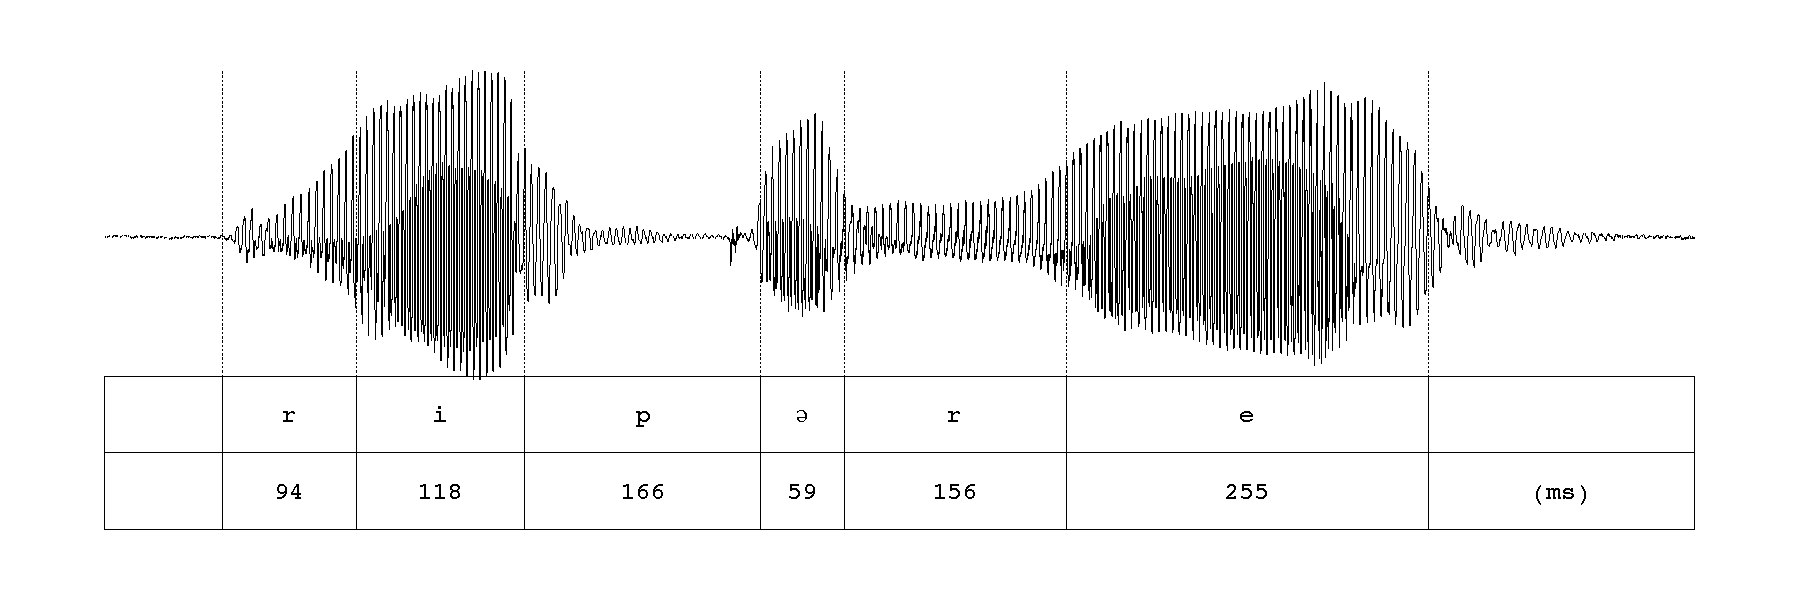
\includegraphics[width=\textwidth]{images/liverNOMSG-1403.pdf}}}
\resizebox{\columnwidth}{!}{%
\fbox{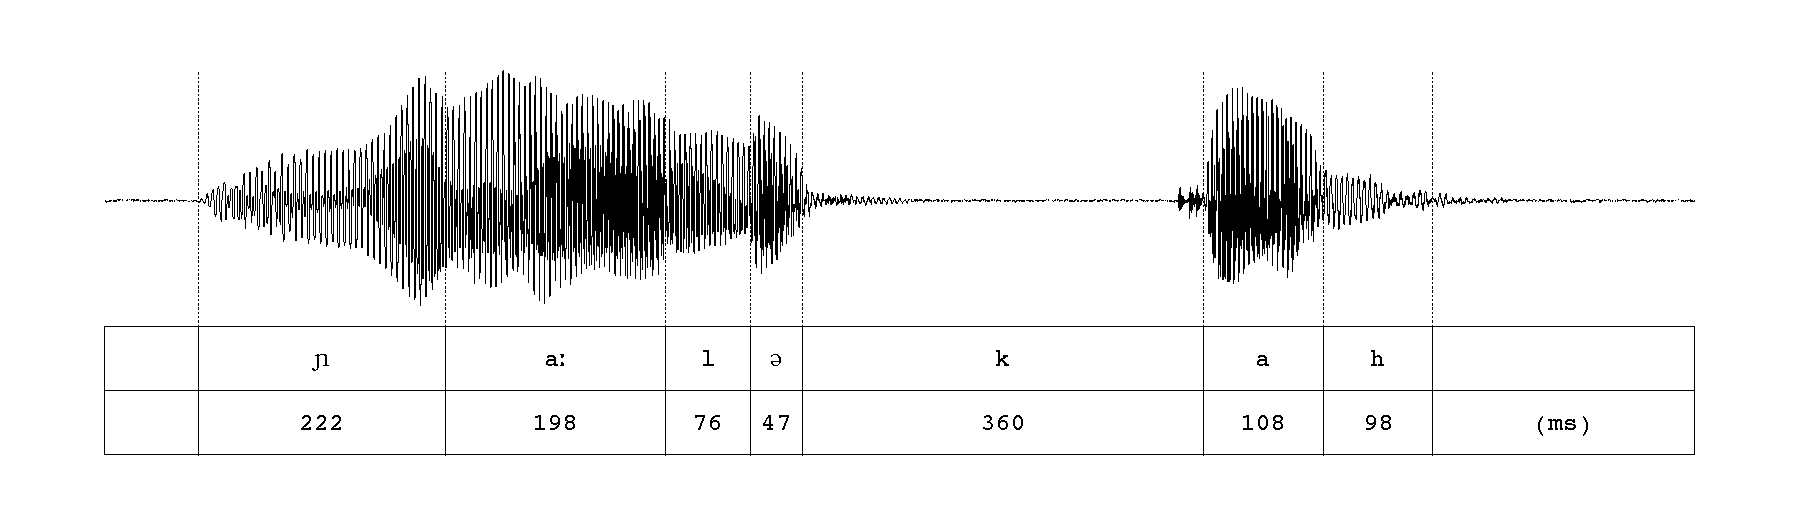
\includegraphics[width=\textwidth]{images/candyNOMSG-1277.pdf}}}
\caption[Waveforms of two words with an epenthetic schwa]{Waveforms of two words (\It{ribbre} ‘liver’ and \It{njálga} ‘candy’) with an epenthetic schwa, including segmental durations}\label{epentheticSchwaWaveforms}
\end{figure}


Speakers are rarely conscious of this vowel, and it is not reflected in the orthography. In neighboring Lule Saami, a similar epenthetic vowel exists and is predictable based on the prosodic and phonological structure of a word \citep[cf.][14-15]{Spiik1989}. It therefore seems likely that this epenthetic schwa is not phonemic in \PS\ either. However, more data is needed to confirm this and thoroughly describe its distribution. The fact that this epenthetic vowel seems to be significantly more prevalent in northern \PS\ dialects complicates the situation further. The examples in \REF{quick} through \REF{whitefishNOMSG} provide dialectal variants, with the more southern variant first (lacking the epenthetic vowel), and the more northern variant second (with the epenthetic schwa).
\ea\label{quick}
\begin{tabular}{p{20mm} x{22mm} l}
\MR{2}{*}{/spaːjːta/} &[spaːjj̥ːta]\textasciitilde	& \It{spájta}	\\
				&[spaːj\Bf{ᵊ}ta] 			& ‘fast’ 		\\
\end{tabular}
\hfill\pbox{\textwidth}{\hfill\small[1711]\\\hfill\hyperlink{pit110518a}{\small[pit110518a.3m22s]}}
\z
\ea\label{deliciousPRED}
\begin{tabular}{p{20mm} x{21mm} l}
\MR{2}{*}{/ɲalːke/} 	&[ɲalːke]\textasciitilde	& \It{njallge}	\\
				&[ɲal\Bf{ᵊ}kːe] 			& ‘tasty’ 		\\
\end{tabular}
\hfill\pbox{\textwidth}{\hfill\small[2323]\\\hfill\hyperlink{pit081111}{\small[pit081111.2m59s]}}
\z
\ea\label{whitefishNOMSG}
\begin{tabular}{p{20mm} x{23mm} l}
\MR{2}{*}{/ʧu͡avːʧa/}	&[ʧu͡aʋːʧa]\textasciitilde	& \It{tjuavvtja}				\\
				&\MR{2}{*}{[ʧu͡oʋ\Bf{ᵊ}ʧa]} 	& ‘whitefish\BS\Sc{nom.sg}’ 	\\
\end{tabular}
\hfill\pbox{.2\textwidth}{\hfill\small[1954]\\\hfill\hyperlink{pit0906_Ahkajavvre_a}{\small[pit0906\_Ahka-}\\\hbox{}\hfill\hyperlink{pit0906_Ahkajavvre_a}{\small javvre\_a.168]}}
\z



%%%%%%% THIS IS NOT USED FOR THE ENTIRE COMPILATION, but only for individual chapters!!!!

\clearpage
\addcontentsline{toc}{chapter}{Bibliography}\label{Bibliography}
\bibliography{PiteGrammarBibSDL}%for bibtex
%\printbibliography%[title=Works Cited]%%for biber!






%%%NAME INDEX doesn’t work!?!? why???
\cleardoublepage\phantomsection%this allows hyperlink in ToC to work
\addcontentsline{toc}{chapter}{Name index}
\ohead{Name index}
\printindex[aut]

\cleardoublepage\phantomsection%this allows hyperlink in ToC to work
\addcontentsline{toc}{chapter}{Language index}
\ohead{Language index}
\printindex[lan]

\cleardoublepage\phantomsection%this allows hyperlink in ToC to work
\addcontentsline{toc}{chapter}{Subject index}
\ohead{Subject index}
\printindex


\end{document}